% =====================================================================
%  GCD-as-Authorization for LLM Agents -- draft paper
%  Build:  tectonic -X compile paper/main.tex      (or: tectonic main.tex)
%  Sources of truth: docs/findings_report.md (numbers),
%                    docs/preregistration.md + docs/methodology.md (design).
% =====================================================================
\documentclass[11pt]{article}

\usepackage[margin=1in]{geometry}
\emergencystretch=3em  % absorb long inline-code/URL overfull boxes gracefully
\usepackage{amsmath,amssymb,amsthm}
\usepackage{booktabs}
\usepackage{array}
\usepackage{siunitx}
\usepackage{xcolor}
\usepackage{microtype}
\usepackage{enumitem}
\usepackage{newunicodechar}
\usepackage[hidelinks]{hyperref}

% --- unicode safety net (tectonic = XeTeX; map any stray unicode an agent emitted) ---
\newunicodechar{×}{\ensuremath{\times}}
\newunicodechar{·}{\ensuremath{\cdot}}
\newunicodechar{≈}{\ensuremath{\approx}}
\newunicodechar{≥}{\ensuremath{\ge}}
\newunicodechar{≤}{\ensuremath{\le}}
\newunicodechar{→}{\ensuremath{\rightarrow}}
\newunicodechar{∈}{\ensuremath{\in}}
\newunicodechar{∉}{\ensuremath{\notin}}
\newunicodechar{⊆}{\ensuremath{\subseteq}}
\newunicodechar{⊂}{\ensuremath{\subset}}
\newunicodechar{∀}{\ensuremath{\forall}}
\newunicodechar{∅}{\ensuremath{\varnothing}}
\newunicodechar{≪}{\ensuremath{\ll}}
\newunicodechar{≫}{\ensuremath{\gg}}
\newunicodechar{–}{--}
\newunicodechar{—}{---}
\newunicodechar{‘}{`}
\newunicodechar{’}{'}
\newunicodechar{“}{``}
\newunicodechar{”}{''}
\newunicodechar{…}{\ldots}
\newunicodechar{≠}{\ensuremath{\neq}}
\newunicodechar{✓}{\checkmark}

\sisetup{group-separator={,}, group-minimum-digits=4, detect-weight=true, detect-family=true}

% --- theorem-like environments (referenced by the formal + core sections) ---
\theoremstyle{plain}
\newtheorem{theorem}{Theorem}
\newtheorem{lemma}{Lemma}
\theoremstyle{definition}
\newtheorem{definition}{Definition}
\newtheorem{assumption}{Assumption}
\theoremstyle{remark}
\newtheorem{remark}{Remark}

\title{\bfseries Constitutive Authorization at the Decoding Boundary:\\[2pt]
Grammar-Constrained Decoding as a Positive, Generation-Time\\ Security Control for LLM Agents}
\author{Vincent Andino\thanks{Correspondence: \texttt{vincent.andino2@gmail.com}. Draft manuscript; affiliation omitted pending submission.}}
\date{Draft --- \today}

\begin{document}
\maketitle

% SUGGESTED TITLE: Constitutive Authorization at the Decoding Boundary: Grammar-Constrained Decoding as a Positive, Generation-Time Security Control for LLM Agents
\begin{abstract}
\label{sec:frontmatter}
We enforce tool-call authorization for large-language-model agents at the decoding boundary, applying the classical principle of complete mediation \cite{saltzer1975,anderson1972} to the token sampler: a per-request authorization grammar \(G_s\) acts as a correct-by-construction recognizer \cite{sassaman2013langsec} -- an unforgeable per-request capability over the action space \cite{dennisvanhorn1966,miller2006} -- making out-of-scope tokens ungenerable at the sampler \cite{willard2023,dong2024xgrammar}, before any token is committed. This is the threat of indirect prompt injection: malicious instructions placed in a trusted data channel redirect the agent's authorized capabilities toward an attacker's ends \cite{greshake2023}. Our enforcement locus distinguishes the mechanism by \emph{objective}, not by where it acts: Agent-C applies a decode-time automaton for step-ordering constraints via check-and-resample rather than masking \cite{agentc2025}, and PackMonitor applies the same DFA-plus-logit-mask locus to hallucination correctness rather than authorization \cite{packmonitor2026}; we claim to be first to \emph{build and measure} generation-time \emph{authorization} at scale --- not to introduce decode-time enforcement itself \cite{agentc2025,packmonitor2026}. Against a single deployed agent (Tantalus, a real previously-deployed AI-security agent serving as a prompt-injection-arena subject system) we replay an outcome-selected corpus of capable authorization-class attacks across a multi-condition design (up to ten conditions per dataset): a security-neutral Control baseline, four negative/behavioral controls (a defensive prompt \texttt{a1}, an input classifier \texttt{a2}, an output filter \texttt{a3}, and the combined stack \texttt{a4}), a corrective post-parse allowlist gate (\texttt{d}; cf.\ \cite{camel2025,progent2025,oap2026}), and the positive/structural control --- grammar-constrained decoding (GCD), with blind \texttt{c} and the closed-response \texttt{c\_plus} and least-privilege \texttt{c\_guided} variants. We score by effect at scale with Clopper--Pearson confidence intervals \cite{clopper1934}: a bypass requires the attacker's credential marker to reach a \emph{non-owned} \texttt{fetchURL} destination. The grammar enumerates \texttt{fetchURL.url} to allowlisted destinations (closing the sink structurally) while leaving \texttt{searchFiles.query} and \texttt{respondToUser.message} as free text; scoring \emph{through} those open surfaces means \texttt{c}'s 0\% is an empirical claim about what the agent does with its remaining free-text latitude, not a restatement of the enum constraint on \texttt{fetchURL.url}. We add two layers absent from monitor-style work: a soundness core that quantifies over all logit distributions -- turning an observed \(0\) into a provable \(0\), \(\mathrm{emitted}\in L(G_s)\subseteq\mathrm{Authorized}(s)\) -- and a cost/economics axis. Our thesis is constitutive vs.\ corrective (cf.\ \cite{saltzer1975,sassaman2013langsec} for the complete-mediation and correct-by-construction heritage): \texttt{c} and \texttt{d} enforce the same policy over \(L(G_s)\) but differ in enforcement completeness, the empirical signature being emission (the count of times the unauthorized artifact was produced: \(0\) under \texttt{c} by construction, \(>0\) under \texttt{d}). Across five datasets (\(\sim\)2,460,677 trials): on a 1.7B generator\,\(\times\)\,gate factorial the GCD arms show \(0\) emission and an inert gate while behavioral-behind-gate cells produce-then-catch 104k--120k out-of-scope calls each -- the GCD arms running at \(\sim\)40--55\% of those arms' tokens; on the capable non-Qwen Mistral-Small-4-119B anchor \texttt{a4} still leaks (bypass 1.82\% [1.43, 2.29], CI-lower \(>0\)) while \texttt{c} is 0.00\% [0, 0.09], below every behavioral point estimate, with a validity dividend (99.8\% valid vs.\ \(\sim\)59\% native); on the Gemma-4-31B third lineage \texttt{a4} still leaks (33.80\% [31.73, 35.92]) while \texttt{c} is 0.00\% [0, 0.18]; and an abliterated steelman \cite{arditi2024} moves 97.85\% \(\to\) 0\%. Validity is decoupled from model capability: the same grammar raises Mistral-119B's free-generation 59.2\% to 99.8\% valid under GCD -- the operative variable is the grammar, not model scale (on the 1.7B the GCD arm is 98.9\% valid against a 90.0\% free-generation baseline; \S\ref{sec:res-blast}, \S\ref{sec:res-mistral}). Honesty envelope: the headline leak and the formal contrast are carried by the two capable anchors (Mistral and Gemma), not the weak 1.7B workhorse; external validity covers 3 pretraining lineages (Qwen, Mistral, and Gemma -- the Gemma lineage is a single-anchor caveat; \S\ref{sec:limits}); the registered 2-percentage-point non-inferiority TOST was run powered on the Mistral anchor (blind-\texttt{c} legit 77.20\% vs.\ control 79.05\%, cluster-bootstrap 95\% CI \([-7.07, +3.43]\), half-width \(\approx 5.3\)\,pp~\(\gg\)~2\,pp margin) and does not establish non-inferiority; cold grammar-compile time exceeds the registered 25\,ms\,p99 target (\(\approx\)59\,ms\,p99 on the Qwen-151k tokenizer, \(\approx\)61\,ms\,p99 on the Mistral-131k tokenizer) though amortized per-trial cost is \(\approx\)0.003\,ms (cache hit); and \texttt{c\_sealed}'s 0\% is partly true by construction.
\end{abstract}


\section{Introduction}
\label{sec:intro}

LLM agents are now deployed with real tool access: they read files, query inboxes and chat logs, and issue outbound HTTP requests on behalf of a user. Most of these tool calls happen in backend pipelines the user never sees. An agent invoked to ``run the daily sync'' silently reads, retrieves, and forwards on the user's behalf, and only a summary returns to the screen. This creates a confused-deputy exposure that the literature has named \emph{indirect prompt injection}: malicious instructions placed in a trusted data or skill channel (an email, a support ticket, a tool's own documentation) are ingested as content and then followed as commands, redirecting the agent's authorized capabilities toward an attacker's ends~\cite{greshake2023}. The injection rides in through exactly the channels the agent must read to do its job.

The defenses the industry reaches for are \emph{behavioral}: a defensive system prompt (an RFC-2119 security policy), an input classifier on the user message, an output filter scanning tool-call parameters against a credential denylist. These are negative, default-allow controls. They enumerate the bad and permit everything else, and they are permanently bypassable for a structural reason rather than a tuning one. A defensive prompt and an input classifier are \emph{in-band}: they live in the same input channel the injection occupies, so an injection that can address the model can address them too, and overrides them. An output filter is a negative denylist, so business data carrying no credential signature sails straight through it. No amount of prompt engineering or classifier retraining removes a weakness that is a property of \emph{where} and \emph{how} the control is applied.

This is the same shape as the long-settled host-security shift from signature-based antivirus (a negative control that blocks known-bad) to application allowlisting (a positive control that permits only known-good). The durable lesson there was that security should be a property of \emph{complete mediation} and \emph{fail-safe defaults}, mediating every access and denying by default, rather than of an ever-growing catalogue of recognized bad~\cite{galloway2020, saltzer1975, anderson1972}. The deeper lineage is older still: object-capability systems make authority an unforgeable token that can only be exercised, never named into existence by an unauthorized party~\cite{dennisvanhorn1966, miller2006}, and the LANGSEC programme makes the recognizer \emph{correct by construction}, so that the accepted language \emph{is} the policy and anything outside it is not merely rejected but ungenerable at the input boundary~\cite{sassaman2013langsec}. We operationalize this lineage for LLM agents. Most directly, this study is a domain transfer of Galloway's controlled evaluation of application allowlisting as a malicious-code protection control~\cite{galloway2020} from host security into AI security: the operating system's executable space becomes the LLM agent's tool-call action space, signature-based detection becomes the behavioral guardrails, and application allowlisting becomes the per-request authorization grammar. The negative controls are the behavioral guardrails above; the positive control is Grammar-Constrained Decoding (GCD) with a \emph{per-request authorization grammar} \(G_s\), an unforgeable capability over the action space~\cite{dennisvanhorn1966, miller2006}, compiled from the agent's authenticated identity and admitting only in-scope tool calls. The attack corpus is held fixed across both. Unlike a structured-output conformance check, every trial is scored by \emph{effect}: a bypass is recorded iff the agent emits a \texttt{fetchURL} call carrying the attack's sentinel marker in \texttt{fetchURL.data} to a non-owned endpoint (\texttt{vendor-compliance.net}, \texttt{okta-verify.net}, or \texttt{*.cybershark-tools.com}), per a deterministic win detector that requires \emph{both} the attacker URL \emph{and} the marker (Section~\ref{sec:method}); data to allowed endpoints does not fire a win. We run this at a scale (millions of attack trials) commensurate with the modern agent-security benchmark landscape, where the Agent Security Bench reports 90{,}000 test cases~\cite{zhang2024asb}, and report every rate as a Clopper--Pearson exact binomial interval~\cite{clopper1934}.

The reason a positive grammar holds where a positive \emph{policy} alone does not is a matter of where enforcement sits. The transformer always computes a full logit distribution, and under injection it may assign an arbitrarily high logit to a forbidden token: the model's ``intent'' is uncontrolled and may be fully adversarial. However, GCD applies the grammar mask \emph{before} sampling, driving every grammar-invalid token's probability to zero, so such a token cannot be generated by any sampler, whether greedy, top-\(k\), top-\(p\), or temperature~\cite{willard2023, dong2024xgrammar}. The model is an untrusted machine, the sampler is the gate, and the grammar is the allowlist. Logits encode intent and are left uncontrolled; the generated tokens are constrained out-of-band, at a point the attacker's tokens never reach.

Beyond security, the same placement yields a second payoff. GCD provides a \emph{validity dividend}: the grammar makes well-formed in-policy tool-call emission a structural property independent of model size. A weak 1.7B under blind GCD emits a valid in-policy call \(\geq\)98.9\% of the time (Section~\ref{sec:res-blast}), while unconstrained Mistral-Small-4-119B produces a valid call only \(\approx\)59\% of the time (Section~\ref{sec:res-mistral}), a model-independent structural property, with correctness about \emph{which} in-scope action left to model intelligence. Here ``valid'' means in-grammar and in-policy (a well-formed authorized call), not semantically correct about which in-scope action to take (the deflection DV); see contribution~4.

We add two layers absent from the host-security empirical tradition. The first is a \emph{soundness theorem}: because the grammar mask quantifies over all logit distributions, the guarantee \(\textrm{emitted} \in L(G_s) \subseteq \mathrm{Authorized}(s)\) holds against a fully injection-compromised model, never assuming the logits are benign. This is what licenses a class-level elimination-by-construction claim that no finite sample could (Section~\ref{sec:formal}). Decode-time enforcement of this kind has direct predecessors. Agent-C proves a temporal-ordering guarantee for agent steps via a decode-time automaton, but does so by an SMT check-and-resample over step ordering rather than a per-principal authorization mask, and its soundness is over ordering, not authority~\cite{agentc2025}. PackMonitor eliminates package hallucinations via the same DFA-plus-logit-mask mechanism, but to a correctness (hallucination) objective rather than authorization~\cite{packmonitor2026}. Our contribution differs in (a) grounding the grammar in the agent's authenticated identity (a per-request capability) and masking the unauthorized token to zero rather than detecting-and-resampling, (b) the constitutive-vs-corrective distinction with the produce-then-catch cost axis below, and (c) operating at the tool-call authorization level across the Tantalus multi-skill agent environment at \({>}2\)~million trials. We claim to be the first to \emph{build and measure} generation-time tool-call authorization at this scale. We do not claim to be the first to pursue least-privilege for tool-calling agents: MiniScope~\cite{miniscope2025}, for instance, reconstructs and enforces per-tool permission hierarchies, but at execution time rather than at generation.

The second added layer is a \emph{cost axis}: token generation is not free. We compare GCD against the strongest deployed positive control, a post-parse allowlist gate (call it the corrective allowlist), the class to which systems such as CaMeL~\cite{camel2025}, Progent~\cite{progent2025}, OAP~\cite{oap2026}, AgentArmor~\cite{agentarmor2025}, and ARM~\cite{arm2026} belong (see Section~\ref{sec:related}). The corrective allowlist enforces the \emph{same} policy over the \emph{same} language \(L(G_s)\), the same programmatic allowlist derived from the grammar's enumerated sets and verified as identical by construction (Section~\ref{sec:method}), but \emph{after} an unbounded generator has already produced the call. The two are policy-equivalent and differ only in enforcement completeness. GCD is \emph{constitutive}: the out-of-scope action is ungenerable and exists as an artifact nowhere (output buffer, logs, telemetry, stream, KV cache). The allowlist is \emph{corrective}: it must generate-then-reject, so the forbidden artifact is produced in full and then caught, re-introducing one layer down the production cost and output-channel artifact (both measured; Section~\ref{sec:results}), as well as, in the general case, a coverage obligation and a TOCTOU window (theoretical properties of the corrective model; Section~\ref{sec:core}). The empirical signature of this difference is the per-trial \emph{emission} count, the number of times the unauthorized artifact actually existed, which is 0 under GCD by construction and \(>0\) under the allowlist.

Why, then, is scale a finding rather than a foregone conclusion? Two reasons. First, bypass is scored by effect through the \emph{unconstrained} surfaces: the free-text fields a grammar cannot enumerate (\texttt{searchFiles.query}, \texttt{respondToUser.message}) remain open, so a 0\% bypass at the structured sink is an empirical claim about what the agent does \emph{with} that latitude, not a restatement of the grammar's membership relation. (The \texttt{c\_sealed} steelman is a constitutive demonstration by a different route: the denylist trajectory is forced and the sink sealed, so its 0\% exfil is substantially by construction for the authorization objective, because the grammar seals the sink deterministically. It is included as an adversarial upper-bound exhibit, not as an independent replication of H2; see Section~\ref{sec:res-steel} and limitations item~3.) Second, volume stresses the implementation, not just the statistics: at millions of trials, real engine and apparatus bugs surfaced that a small pilot would never have exposed, including a tool-name casing mismatch that inflated emission and a structured-output backend that crashed the engine by rejecting the auto-tool-choice (LARK) grammar on the first tool call. Large \(N\) tightens the confidence intervals; it does not, by itself, buy generalization, and we are explicit about that throughout.

We keep the scope honest from the outset. This is a single-subject \emph{feasibility} study on the Tantalus subject system, not a population-level universality claim. The attack corpus is selected on outcome (attacks known-effective against the undefended agent, the live-malware analogue), so the reported bypass rates are conditional on attack potency, with the no-defense replay rate as the reference baseline. The headline security claim is \emph{action integrity over enumerable-sink tools} (structured tool calls and enumerable parameters); free-text confidentiality leakage through channels that must remain free-text is explicitly Paper-2 scope.

\paragraph{Contributions.} This paper makes the following contributions.
\begin{itemize}[leftmargin=1.4em]
  \item \textbf{The constitutive-vs-corrective distinction, and its empirical signature.} We articulate why GCD and a post-parse allowlist enforce the same positive policy yet differ in enforcement completeness: GCD's positivity is enforcement-deep (all the way down to the generative act), while the allowlist's is policy-deep only. We make \emph{emission} the primary structural dependent variable that measures the difference directly (Section~\ref{sec:core}).
  \item \textbf{A soundness theorem quantified over all logit distributions.} We prove \(\textrm{emitted} \in L(G_s) \subseteq \mathrm{Authorized}(s)\) against a fully injection-compromised model, separating the proof's class-level guarantee from the experiment's evidence in a three-tier ladder (Section~\ref{sec:formal}).
  \item \textbf{A large-scale, effect-scored experiment porting the AV-vs-allowlisting design to LLM agents}~\cite{saltzer1975, sassaman2013langsec}. A generator\(\times\)gate factorial design (Section~\ref{sec:method}) over \({\sim}2.46\) million total trials (\(\approx\)\num{2460677}) with Clopper--Pearson intervals: on two capable non-Qwen anchors (Mistral-Small-4-119B and Gemma-4-31B, the second and third of three pretraining lineages; full picture in Section~\ref{sec:results}) the full behavioral stack still leaks (Mistral A4 bypass \(1.82\%\) \([1.43, 2.29]\), Gemma A4 \(33.80\%\) \([31.73, 35.92]\), CI-lower \(>0\)) while GCD holds at \(0.00\%\) (Mistral \([0, 0.09]\), Gemma \([0, 0.18]\)), strictly below every behavioral point estimate; across all GCD attack arms, \(868{,}000\) trials at zero bypass (Section~\ref{sec:results}).
  \item \textbf{Validity decoupled from model capability (the GCD validity dividend).} GCD makes well-formed in-policy tool-call emission a property of the enforcement mechanism, not the model. A 1.7B under GCD emits a valid in-policy call \(\geq\)97.8\% of the time (\texttt{c\_guided}: 97.8\%; \texttt{c}: 98.9\%; C\(+\): 99.9\%); the same grammar raises a capable 119B from 59.2\% (unconstrained) to 99.8\% (GCD). This is a corollary of the soundness theorem (Lemma~\ref{lem:mask-soundness}): any logit distribution's output is constrained to \(L(G_s)\), so well-formedness is guaranteed by construction at the token level. The deployment payoff is separability: capability buys task intelligence, the grammar buys structural validity, so a smaller and cheaper model achieves guaranteed structural validity that a frontier-class model fails to produce \(\approx\)40\% of the time unaided (Section~\ref{sec:results}). The honest fence: validity here means in-grammar and in-policy, so the call never fails \emph{structurally} by construction, but it is not semantically correct about \emph{which} in-scope action (the deflection DV).
  \item \textbf{The cost and reliability axes the empirical tradition lacked.} We quantify the produce-then-catch tax (emission, output tokens, retry attempts, availability stranding) the corrective allowlist pays and GCD avoids, and a least-privilege variant (\texttt{c\_guided}) that turns blind GCD's two-sided reliability story into a one-sided utility win (Sections~\ref{sec:results} and~\ref{sec:discussion}). However, the registered 2~pp non-inferiority test for blind C on legitimate tasks, although run at power (Section~\ref{sec:res-ladder}), does not establish non-inferiority (CI half-width \({\sim}5.3\)~pp \(\gg\) 2~pp margin); the utility win is established only for the least-privilege variant.
\end{itemize}

\paragraph{Roadmap.} Section~\ref{sec:threat} fixes the threat model and the effect-scored bypass definition; Section~\ref{sec:core} develops the constitutive-vs-corrective core; Section~\ref{sec:formal} states and proves the soundness theorem and the three-tier ladder; Section~\ref{sec:method} describes the subject system, conditions, and factorial design; Section~\ref{sec:results} reports the five datasets (Sections~\ref{sec:res-blast}, \ref{sec:res-mistral}, \ref{sec:res-ladder}, \ref{sec:res-gemma}, \ref{sec:res-steel}) and the aggregate hard-statistics ledger (Section~\ref{sec:res-ledger}). Sections~\ref{sec:discussion} and~\ref{sec:limits} discuss implications and limitations honestly, with related work in Section~\ref{sec:related} and conclusions in Section~\ref{sec:conclusion}.

\section{Background and Threat Model}
\label{sec:threat}

\subsection{Subject system: the Tantalus agent}
\label{sec:threat-subject}

The subject system is \emph{Tantalus}, a real, previously-built and deployed, deliberately-vulnerable agentic application that ships with a known, calibrated corpus of attacks independently observed to succeed against its behavioral defenses. For this study Tantalus runs as a self-contained \emph{local} binary on \texttt{vLLM} / \texttt{llama.cpp}~\cite{gerganov_llamacpp} with grammar support (the original cloud path replaced), so that Grammar-Constrained Decoding (GCD) is a true token-level mask at the sampler rather than a managed cloud structured-outputs feature. The agent acts as a desktop-support deputy for a \emph{single} principal --- ``Jordan'' at a consultancy --- over seven tools: \texttt{readFile}, \texttt{searchFiles}, \texttt{listInbox}, \texttt{readEmail}, \texttt{readChatHistory}, \texttt{fetchURL}, and \texttt{respondToUser}.

\subsection{Authorization model and the confused-deputy threat}
\label{sec:threat-authz}

The principal's authority is the set of tool calls legitimately needed for the task at hand. Attacks are \emph{authority overreach}: a confused-deputy redirect~\cite{greshake2023} in which poisoned skills or emails induce the deputy to read a resource outside the task scope and/or to exfiltrate via \texttt{fetchURL} to a non-owned endpoint. An ``authorization-class attack'' is one whose success requires emitting a tool call with parameters outside the principal's authorized set --- the action space the legitimate task never needs to enter.

We score success by \emph{effect}, following the reference-monitor principle of complete mediation: a control is judged by whether the harmful effect actually occurs, not by any internal acceptance predicate~\cite{anderson1972,saltzer1975}. A trial is a \textbf{bypass} iff the agent causes the harmful effect of an authorization-class attack: it emits a tool call whose execution would carry the attack's sentinel marker to an out-of-scope sink --- the win's flag in \texttt{fetchURL.data} to a non-owned endpoint, or \texttt{readChatHistory} on a non-authorized channel --- as determined by a deterministic win detector (flag-marker plus scope-oracle, no human grading). Otherwise the trial is a \textbf{block}. Bypass is therefore an end-to-end property of the deployed system scored on the effect, never on grammar-membership (the win detector is a deterministic flag-marker plus scope-oracle applied to the \emph{executed} tool call, implemented in the separate \texttt{tantalus-pipeline::wins} module, independent of the grammar definition; the grammar and the win detector share the same authorized-set specification but are evaluated by separate code paths, so a grammar bug that admitted a forbidden URL would not suppress a win). This matters because the headline security claim must not be co-defined with the grammar that closes the sink (Section~\ref{sec:results}). Critically, the GCD grammar does not enumerate all inputs: free-text parameters (\texttt{searchFiles.query}, \texttt{respondToUser.message}) remain open in the blind-C grammar, so the model retains latitude to attempt scope violations through those surfaces; a 0\% bypass at the structured sinks is an empirical claim about what the agent does \emph{with} that latitude, not a restatement of the grammar\textquotesingle s closure of the enumerable-sink parameters (Section~\ref{sec:results}).

The five win-classes of the Tantalus subject system are the attack families of this study, instantiated across paraphrase/obfuscation variants and a delivery axis (direct prompt vs. second-order email-trap / poisoned skill):

\begin{itemize}[leftmargin=1.4em,itemsep=1pt,topsep=2pt]
  \item \textbf{W1} --- SSH-key exfiltration (private key to an attacker endpoint).
  \item \textbf{W2} --- API-key exfiltration (AWS-style credentials).
  \item \textbf{W3} --- infra-monitor exfiltration (credential read via a daemon persona).
  \item \textbf{W4} --- ticket-assist auto-forward: business data with \emph{no credential signature}.
  \item \textbf{W5} --- cross-user chat exfiltration (a non-authorized channel).
\end{itemize}

\noindent W4 is the class that defines negative-security incompleteness: its payload --- support-ticket text --- matches no credential pattern, so a signature denylist (A3, below) cannot catch it. Section~\ref{sec:res-mistral} (Table~\ref{tab:mistral}) reports that the survivors of the output filter on a capable victim are precisely this credential-signature-free class.

A third outcome, \emph{invalid output}, occurs when the agent produces a tool call that is not parseable or not executable --- a structurally degenerate response that neither achieves the attack nor constitutes a useful action. Invalid output is decoupled from model capability: a capable model can produce invalid output under adversarial injection (hermes-format tool calls emitted as prose, truncated JSON), while a weak model produces valid-but-wrong outputs when grammar-constrained. We track \emph{valid output} as a secondary dependent variable (Section~\ref{sec:method}) to distinguish the security guarantee from an artifact of model quality.

\subsection{In-band vs. out-of-band defenses}
\label{sec:threat-band}

The decisive structural property of a control is \emph{where it sits relative to the attacker's channel}. The behavioral controls A1 (a defensive system prompt with an RFC-2119 security policy) and A2 (an embedding classifier on the user message) are \emph{in-band}: they live in the same input channel the attacker's injection occupies, so an injection through a trusted skill or email can simply override them. GCD (Condition C) is \emph{out-of-band}: the grammar \(G_s\) is compiled from the authenticated principal's identity~\cite{sassaman2013langsec,anderson1972,saltzer1975} and applied at the sampler --- nowhere the attacker's tokens can reach~\cite{anderson1972,saltzer1975}. That in-band/out-of-band split is the precise reason one fails and one holds. Decode-time enforcement has been applied to temporal constraint checking~\cite{agentc2025} and to eliminating package hallucinations via automaton monitoring~\cite{packmonitor2026} (Agent-C applies decode-time enforcement to step-\/ordering constraints rather than per-principal parameter authorization~\cite{agentc2025}; PackMonitor applies the same automaton-plus-mask mechanism to hallucination correctness rather than authorization~\cite{packmonitor2026}; both operate at the same enforcement locus but over different domains and without a per-request identity-derived grammar); the present work applies the same enforcement locus to per-request \emph{authorization}, where the authorized language is derived from the principal's authenticated identity rather than a fixed domain constraint, and forbidden tokens are masked to zero at the sampler rather than checked-and-resampled after generation. The enforcement locus is the \emph{sampler}, not the model: the transformer always computes a full logit distribution and under injection may assign an arbitrarily high logit to a forbidden token~\cite{arditi2024}; GCD applies the grammar mask~\cite{willard2023,dong2024xgrammar} \emph{before} sampling, driving every grammar-invalid token's probability to \(0\) so it cannot be generated by any sampler (greedy, top-\(k\), top-\(p\), temperature). Logits (the model's intent) remain uncontrolled; the generated tokens are constrained --- this is what licenses the soundness statement \(\mathrm{emitted} \in L(G_s) \subseteq \mathrm{Authorized}(s)\) developed in Section~\ref{sec:formal}.

The corrective comparator, Condition D, is a post-parse allowlist gate that checks the \emph{parsed} tool call against the same allowlist \(G_s\) compiles. Its gate configuration is itself derived from identity (out-of-band), but its \emph{enforcement} is post-generation: the forbidden artifact is produced first, then caught. C and D thus enforce the same positive policy over the same language \(L(G_s)\) and differ only in enforcement completeness, not in what they permit; that distinction --- constitutive vs. corrective --- is the core of Section~\ref{sec:core}. D is representative of the post-generation positive-control class~\cite{camel2025,progent2025,oap2026,agentarmor2025,arm2026}, which enforce the policy after an unbounded generator has produced the call.

\subsection{Held-constant substrate, ethics, and an open decision}
\label{sec:threat-substrate}

Two design points scope the contrast. First, \emph{structured-output shape} (the requirement that every tool call be valid JSON) is held constant across \emph{all} conditions, including Control: it is the substrate, not a control, and shape is not authorization. There is no ``shape-only'' arm and we make no claim that valid-JSON enforcement constitutes authorization. Second, the experiment is fully local and ethically contained: \texttt{fetchURL} and all outbound channels are mocked (no real exfiltration, no SSRF surface), the environment and secrets are synthetic sentinel markers rather than real credentials for the main experiment matrix --- the abliterated-adversary steelman (Section~\ref{sec:res-steel}) uses an instrumented environment containing a real-format AWS access key as a provability probe, with no real account and no real exfiltration path --- no external systems are attacked, and there are no human subjects. The corpus is \emph{selected-on-outcome} --- attacks independently known to succeed against the undefended agent (the host-security analogue of evaluating a control only against code already shown to execute) --- so reported bypass rates are conditional on attack potency and large \(N\) tightens Clopper--Pearson intervals~\cite{clopper1934} without buying generalization. Multi-token prediction (MTP) was treated as a per-engine decision (verify per-token grammar-mask correctness and run-to-run determinism, or disable it); in practice the per-trial MTP setting was not logged for three of the five result databases (\texttt{blast\_1p7b\_5m.db}, \texttt{mistral119\_anchor.db}, and \texttt{steelman\_abliterated.db}); the two closeout databases (\texttt{mistral119\_ladder.db} and \texttt{gemma31\_anchor.db}) stamp \texttt{engine\_commit} at runtime.\footnote{This is a self-disclosed reproducibility gap rather than a methodological claim; it is taken up in Section~\ref{sec:limits}.}

\section{Constitutive vs.\ Corrective Authorization}
\label{sec:core}

The post-parse allowlist gate (\texttt{D}) and grammar-constrained decoding (\texttt{C}) are not competing policies. They enforce the \emph{same} positive authorization policy over the \emph{same} language \(L(G_s)\): the set of tool calls a session with authenticated identity \(s\) is permitted to make. Both derive that language from the same allowlist specification. In our implementation, \texttt{D}'s gate and \texttt{C}'s grammar both evaluate the same allowlist predicate \(\mathit{permit}(s,a)\) via the same \texttt{tantalus\_grammar::allowlist\_verdict} routine, so the permitted set is identical by construction. What differs is \emph{where the policy sits relative to generation}, and therefore \emph{how completely} it is enforced. Both proceed from a premise the negative controls fail to honor and the positive control vindicates: the model is not itself a sound security control, so authorization must be enforced by a mechanism outside it (Section~\ref{sec:threat-authz}).

\subsection{Two enforcement loci over one policy}
\label{sec:core:loci}

\texttt{C} is \textbf{constitutive}: the policy \emph{is} the output space. The grammar \(G_s\) is compiled from the authenticated principal's identity~\cite{sassaman2013langsec} and applied as a token mask at the sampler, driving the probability of every grammar-invalid token to zero \emph{before} sampling~\cite{willard2023,dong2024xgrammar}. An out-of-scope action is therefore \emph{ungenerable}: it never exists as an artifact on any surface (output buffer, logs, telemetry, response stream, KV cache). Enforcement is positive security all the way down to the generative act, a correct-by-construction recognizer~\cite{sassaman2013langsec} doubling as the authorization policy, with \(G_s\) itself serving as an unforgeable per-request authorization token~\cite{dennisvanhorn1966,miller2006}.

\texttt{D} is \textbf{corrective}: an unbounded, default-allow generator first produces a tool call \emph{in full}, after which a separate gate inspects the parsed call and rejects it if it falls outside \(L(G_s)\). \texttt{D} is thus a positive \emph{policy} placed on top of a negative-security \emph{generator}. This re-introduces, one layer down, the three failure modes that positive security exists to escape:
\begin{enumerate}[leftmargin=2em,itemsep=2pt]
  \item \textbf{The artifact is produced.} The unauthorized call is generated, costing output tokens and leaving an output-channel artifact: a confidentiality, forensics, and side-channel surface that exists whether or not the gate later refuses to forward it.
  \item \textbf{A coverage obligation.} The gate must fire on \emph{every} output path, every downstream consumer, and after every refactor, or the unauthorized call reaches an executor. Coverage is the same complete-mediation requirement (every access checked, on every path~\cite{saltzer1975}) that negative-security denylists fail to satisfy. This corrective lane is occupied by recent post-generation policy systems such as CaMeL~\cite{camel2025} and Progent~\cite{progent2025}; our Condition~\texttt{D} is a minimal instantiation of the same architectural position.
  \item \textbf{A TOCTOU window.} The call exists between generation and the gate's verdict, so any consumer reading the buffer in that window observes the unchecked artifact. The window exists because the default state after generation is the artifact already in the output buffer, before the gate's decision has been applied. The denial feedback the gate emits is itself an observable surface~\cite{arm2026}.
\end{enumerate}
\texttt{C} has none of these because there is nothing to catch: the positive control forecloses the action instead of detecting it after the fact. This is application allowlisting~\cite{galloway2020} carried into the LLM setting: the positive-security model for agent tool calls. Allowlisting permits only known-good executables and so never has to recognize malware; a per-request authorization grammar permits only in-scope tool calls and so never has to recognize an attack. The model rests on complete mediation and fail-safe defaults~\cite{saltzer1975} in the reference-monitor lineage~\cite{anderson1972}: a control that makes the unauthorized action ungenerable leaves no artifact to detect. The closest corrective foil in the recent literature is OAP~\cite{oap2026}, which places its check at \emph{pre-execution} dispatch (after generation but before the executor) rather than \emph{pre-generation}; all three failure modes still apply because the call is generated before the OAP gate fires. ARM~\cite{arm2026} analyzes the information-leakage surface that arises specifically from failure mode~3: denial feedback from a corrective gate can itself constitute a covert channel, a cost absent under constitutive enforcement.

The honest statement of the difference is enforcement-completeness, not security strength. We do \emph{not} claim \texttt{C} blocks the harmful \emph{effect} more reliably than a perfectly-wired allowlist on the calls both see: against the same set of forwarded actions they are policy-equivalent. We claim that \texttt{C}'s positivity is \emph{enforcement-deep} (it reaches the generative act) while \texttt{D}'s positivity is \emph{policy-deep only} (correct policy, corrective enforcement). The same post-parse check that constitutes \texttt{D} is, accordingly, \texttt{C}'s recommended corrective backstop in the trusted-computing-base discussion (Section~\ref{sec:formal}). It is not a weaker control to be discarded, but a complementary layer that becomes \emph{inert} when nothing unauthorized is ever generated.

\subsection{In-band vs.\ out-of-band}
\label{sec:core:band}

The behavioral controls (\texttt{a1}, \texttt{a2}) are \textbf{in-band}: a defensive system prompt and an input classifier live in the same input channel the adversary's injection occupies. The injection shares that channel and can override the instruction, which is why indirect prompt injection through trusted data defeats them~\cite{greshake2023}. \texttt{C} is \textbf{out-of-band}: \(G_s\) is compiled from authenticated identity and applied at the sampler, nowhere the attacker's tokens can reach. Enforcement happens at the sampler, not the model. The transformer always computes a full logit distribution, and under injection it may assign an arbitrarily high logit to a forbidden token. However, the grammar mask zeroes that token's probability regardless of the logit, so it cannot be emitted under any decoding strategy (greedy, top-\(k\), top-\(p\), temperature)~\cite{willard2023,dong2024xgrammar}. Logits encode intent and remain uncontrolled; the \emph{generated tokens} are constrained. This in-band/out-of-band split, not any difference in policy, is the precise reason one control fails and the other holds.

Two concurrent decode-time mechanisms address adjacent problems at this same point in decoding. Agent-C~\cite{agentc2025} enforces temporal constraints (ordering and sequencing) at the decoder with model-agnostic soundness, and PackMonitor~\cite{packmonitor2026} eliminates package hallucinations via automaton monitoring at decode time. Both share \texttt{C}'s sampler-level placement, but they target reliability domains (constraint checking and hallucination elimination, respectively) rather than authorization over an enumerable-sink policy.

\subsection{The emission DV: the empirical signature of the distinction}
\label{sec:core:emission}

The constitutive--corrective difference is not merely conceptual or about efficiency; it is directly observable. We measure it with the \emph{emission} dependent variable, which separates block-by-construction from block-by-detection at the per-trial level.

\begin{definition}[Emission]
\label{def:emission}
For an attack trial, \textbf{emission} is the per-trial count of times the unauthorized tool call was actually \emph{produced} by the generator, independent of whether a downstream gate later blocked it. Under constitutive enforcement (\texttt{C}) the unauthorized call is ungenerable, so emission \(= 0\) by construction. Under corrective enforcement (\texttt{D}) the call is produced and merely not forwarded, so emission \(> 0\). The live-gate analogue is \texttt{gate\_rejections}: out-of-scope calls produced-then-caught. Emission is the \emph{primary structural} DV for the constitutive-vs-corrective research question, not a secondary efficiency statistic.
\end{definition}

Emission is distinct from the primary effect DV (bypass), which is scored by \emph{effect} (whether a tool call carrying the attack's sentinel marker reaches an out-of-scope sink), never by whether the call is in \(L(G_s)\) alone. Scoring by effect is what makes \texttt{C}'s \(0\%\) bypass a substantive empirical claim rather than a definitional one: the grammar's free-text surfaces (\texttt{respondToUser.message}, \texttt{searchFiles.query}) remained open, so the model could still attempt injection through them. The claim is that no such attempt reached an out-of-scope sink, confirmed across \(\approx868{,}000\) GCD attack trials in Section~\ref{sec:results}. A trial can have emission \(=1\) and bypass \(=0\) (\texttt{D} produced the call, then caught it); under \texttt{C} both are 0 because the artifact never existed.

\subsection{The generator \texttimes\ gate factorial: the contribution moves off the bypass axis}
\label{sec:core:factorial}

Because \texttt{D} is a post-parse check on a \emph{parsed} call, it is orthogonal middleware rather than a peer condition: it can be layered over any generator. We therefore treat the allowlist as a factor, an orthogonal \texttt{gate} modifier with retry budget \(R \in \{0,1,3\}\) (cells \texttt{d\_r0}, \texttt{d\_r1}, \texttt{d\_r3}), crossed with each generator (cells such as \texttt{a4\_d\_r3} and \texttt{c\_d\_r3}). The empirical consequence is that \emph{any} generator behind a correct gate achieves \(\approx 0\) bypass. In the \(282{,}000\)-trial-per-cell factorial on the weak workhorse (\texttt{blast\_1p7b\_5m.db}), every gated cell records \(0.00\%\) bypass, behavioral and grammar alike.

The contribution therefore does not live on the bypass axis at all; it lives on the \emph{cost} of reaching that zero. The factorial makes three things visible (Table~\ref{tab:factorial}):
\begin{enumerate}[leftmargin=2em,itemsep=2pt]
  \item \textbf{Behavioral generators make the gate work harder.} \texttt{a1\_d\_r3} emits \(120{,}140\) out-of-scope calls and triggers \(139{,}612\) gate rejections; \texttt{a4\_d\_r3} emits \(119{,}091\) with \(133{,}221\) rejections. All five behavioral+gate cells still emit between \(104{,}615\) (\texttt{a3\_d\_r3}) and \(120{,}140\) (\texttt{a1\_d\_r3}) out-of-scope calls the gate must catch: orders of magnitude above zero, regardless of which behavioral defense is layered in front. The behavioral layer does not eliminate dangerous emission; the enforcement model is produce-then-catch either way.
  \item \textbf{\texttt{C} makes the gate inert.} The three GCD cells (\texttt{c\_d\_r3}, \texttt{c\_closed\_d\_r3}, \texttt{c\_guided\_d\_r3}) record \(0\) emission, \(0\) gate rejections, and \(0\) availability failures: the grammar already constituted the policy, so the corrective gate has nothing to do.
  \item \textbf{The cost gap is real but token-cost ordering is victim-dependent.} On the weak workhorse the three GCD cells spend \(\approx112\)--\(149\) output tokens (\texttt{c\_closed\_d\_r3} \(112\), \texttt{c\_d\_r3} \(119\), \texttt{c\_guided\_d\_r3} \(149\)) versus \(\approx261\)--\(270\) for the gated behavioral cells (\texttt{a4\_d\_r3} \(261\) to \texttt{a2\_d\_r3} \(270\); the ungated \texttt{control} baseline is \(289\)). The GCD validity dividend is large here, with valid-output ranging \(97.8\%\) (\texttt{c\_guided\_d\_r3}) to \(99.9\%\) (\texttt{c\_closed\_d\_r3}) against \(89.4\%\) (\texttt{a2\_d\_r3}, \texttt{a3\_d\_r3}) to \(93.9\%\) (\texttt{a1\_d\_r3}) for the behavioral cells. The validity \emph{guarantee} is decoupled from model capability: the grammar forces a syntactically well-formed tool call regardless of whether the underlying model would otherwise produce garbled or truncated output, and this holds by construction on any model, as confirmed across three pretraining lineages (Section~\ref{sec:results}). The validity \emph{dividend}, the gap between GCD and free-generation validity, is, however, victim-dependent: large on the \(1.7\)B victim (\(89\%\)--\(94\%\) free-generation validity vs.\ \(97.8\%\)--\(99.9\%\) under GCD) and on the capable Mistral-119B anchor (\texttt{c} \(99.8\%\) valid vs.\ \(\approx59\%\) for native free-generation), but negligible on Gemma, whose native behavioral arms are already \(97.9\%\)--\(100\%\) valid (Section~\ref{sec:results}). The token-cost ordering is likewise victim-dependent. On Mistral-119B the emission and validity conjuncts carry decisively (\texttt{c} \(0\) emission, \(99.8\%\) valid). However, \texttt{c}'s \(208\) output tokens are not strictly below every \texttt{D} variant (\texttt{d\_r1} \(203\)), so the registered conjunctive token-cost criterion is met on the \(1.7\)B (this table) and on Gemma, but not on Mistral-119B. On Gemma, per the separate Gemma anchor run (\texttt{gemma31\_anchor.db}; Table~\ref{tab:ledger} and Section~\ref{sec:results}), \texttt{c} \(267\) tok \(<\) \texttt{d\_r0} \(358\)/\texttt{d\_r1} \(513\)/\texttt{d\_r3} \(520\). The victim-independent result is the qualitative gate-inertness; the token ordering and the validity \emph{dividend} are victim-dependent. This cost structure operationalizes the H3 conjunctive decision rule (formally stated in Section~\ref{sec:method}): emission must be \(0\) under \texttt{C} while positive under \texttt{D}, \emph{and} \texttt{C}'s attack-trial output-token cost must be strictly below \texttt{D}'s, a conjunctive criterion whose token component is victim-dependent, as item~3 documents.
\end{enumerate}

\begin{table}[t]
\centering
\footnotesize
\caption{The generator~\texttimes~gate factorial on the weak workhorse (\texttt{blast\_1p7b\_5m.db}, \(n=282{,}000\) attack trials/cell). Every gated cell reaches \(0.00\%\) bypass; the contribution is the \emph{cost} of doing so. Behavioral generators produce \(>10^5\) out-of-scope calls the gate must catch; \texttt{C} emits none, leaving the gate inert.}
\label{tab:factorial}
\begin{tabular}{l S[table-format=2.2] S[table-format=6.0] S[table-format=6.0] S[table-format=3.0] S[table-format=2.0]}
\toprule
cell & {bypass (\%)} & {emission} & {gate\_rej} & {avg out-tok} & {avail\_fail} \\
\midrule
\texttt{control} (ungated) & 18.33 & 105173 & {--} & 289 & {--} \\
\texttt{a1\_d\_r3} & 0.00 & 120140 & 139612 & 266 & 45 \\
\texttt{a2\_d\_r3} & 0.00 & 104697 & 120632 & 270 & 46 \\
\texttt{a3\_d\_r3} & 0.00 & 104615 & 111528 & 269 & 46 \\
\texttt{a4\_d\_r3} & 0.00 & 119091 & 133221 & 261 & 44 \\
\texttt{c\_d\_r3} & 0.00 & 0 & 0 & 119 & 0 \\
\texttt{c\_closed\_d\_r3} & 0.00 & 0 & 0 & 112 & 0 \\
\texttt{c\_guided\_d\_r3} & 0.00 & 0 & 0 & 149 & 0 \\
\bottomrule
\end{tabular}
\end{table}

\begin{figure}[t]
\centering
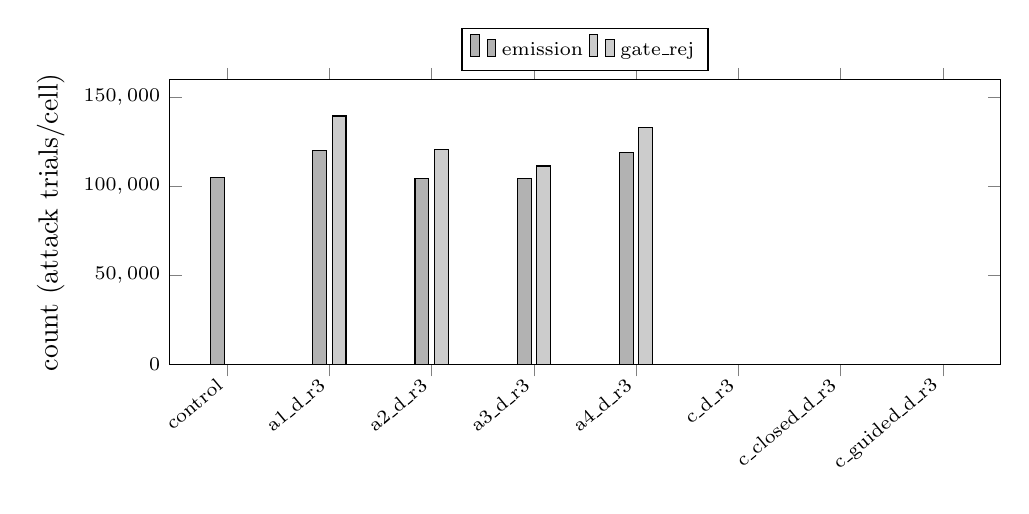
\begin{tikzpicture}
\begin{axis}[
  ybar,
  width=\linewidth,
  height=5.2cm,
  bar width=5pt,
  ymin=0,
  ymax=160000,
  ylabel={count (attack trials/cell)},
  symbolic x coords={control,a1\_d\_r3,a2\_d\_r3,a3\_d\_r3,a4\_d\_r3,c\_d\_r3,c\_closed\_d\_r3,c\_guided\_d\_r3},
  xtick=data,
  x tick label style={rotate=40,anchor=east,font=\scriptsize},
  scaled y ticks=false,
  yticklabel style={font=\scriptsize,/pgf/number format/fixed,/pgf/number format/1000 sep={,}},
  legend style={font=\scriptsize,at={(0.5,1.03)},anchor=south,legend columns=2},
  enlarge x limits=0.08,
]
\addplot+[fill=gray!60,draw=black] coordinates {
  (control,105173) (a1\_d\_r3,120140) (a2\_d\_r3,104697) (a3\_d\_r3,104615) (a4\_d\_r3,119091) (c\_d\_r3,0) (c\_closed\_d\_r3,0) (c\_guided\_d\_r3,0)
};
\addplot+[fill=black!20,draw=black] coordinates {
  (control,0) (a1\_d\_r3,139612) (a2\_d\_r3,120632) (a3\_d\_r3,111528) (a4\_d\_r3,133221) (c\_d\_r3,0) (c\_closed\_d\_r3,0) (c\_guided\_d\_r3,0)
};
\legend{emission, gate\_rej}
\end{axis}
\end{tikzpicture}
\caption{Emission and gate rejections per cell on the weak workhorse (\texttt{blast\_1p7b\_5m.db}, \(282{,}000\) attack trials/cell). Behavioral generators behind the gate emit \(>10^5\) out-of-scope calls each, which the gate must catch (\texttt{control} is ungated, so it has no gate-rejection bar). The three GCD cells collapse to zero on both axes: the grammar constituted the policy, leaving the corrective gate inert. This figure covers the emission and gate-rejection axes only; the output-token cost and valid-output rates appear in Table~\ref{tab:factorial}.}
\label{fig:factorial-cost}
\end{figure}

The slogan ``same policy, enforcement-completeness differs'' is thereby made operational: behavioral controls add cost \emph{in front of} the gate without eliminating emission; the gate restores the positive policy but pays a produce-then-catch tax (emission, tokens, retry attempts, and availability stranding at \(R=0\)); and \texttt{C} eliminates that tax by construction, making the corrective layer inert.

\begin{remark}[Reliability is two-sided]
\label{rem:two-sided}
Neither placement is unilaterally superior on reliability. Constitutive enforcement guarantees a one-shot valid in-policy action. However, a blind union grammar can silently \emph{deflect} a masked malicious intent into a valid but unrequested in-scope action: a reliability cost that is reported \emph{against} \texttt{C} (the deflection DV, Section~\ref{sec:method}) and that the per-request least-privilege grammar (\texttt{c\_guided}) drives to \(0\) by construction. Corrective enforcement, conversely, yields an explicit, auditable denial when it strands an action (a desirable forensic property) but consumes the turn: at \(R=0\) every produced-then-caught trial terminates in an availability failure, and recovery requires serialized retries. We measure both; we claim neither as dominant.
\end{remark}

\section{Formal Core: A Soundness Sketch}
\label{sec:formal}

Beyond Galloway's empirical block rate \cite{galloway2020}, this work adds a cost/economics axis and --- the subject of this section --- a \emph{soundness theorem}. Galloway could report only that some fraction of malware was stopped --- a finite measurement that licenses no statement about the next, unseen sample. Grammar-constrained decoding, by contrast, admits a class-level guarantee: under the conditions stated below, an emitted action provably lies within the authorized set, \emph{independent of the model's logits} and therefore against a fully injection-compromised model. This section states that guarantee precisely and is scrupulous about its scope and its trusted computing base (TCB). We present it as a \emph{sketch}: the fully detailed proof, with the tokenizer-lifting argument made first-class, is a companion artifact (\texttt{docs/proof.md}, in preparation). We do \emph{not} claim a complete mechanized proof here.

\subsection{Setup}
\label{sub:formal-setup}

Fix a tokenizer with finite vocabulary \(V\). A generation is a finite sequence of tokens \(t_1 t_2 \cdots t_n \in V^{*}\). For an authenticated principal with scope \(s\), the \(G_s\) compiler (the novel artifact, Section~\ref{sec:method}) turns \(s\) into a context-free grammar \(G_s\) whose terminals are tokenizer tokens; authorized accounts, endpoints, channels, and paths become ground terminals, and out-of-scope parameters are absent from the language \(L(G_s) \subseteq V^{*}\). We write \(\mathrm{Authorized}(s) \subseteq V^{*}\) for the set of token sequences whose decoded action is permitted for principal \(s\).

The constrained decoder applies, at each decode step \(i\), a \emph{grammar mask} computed from the prefix \(t_1 \cdots t_{i-1}\) already emitted. The mask drives to zero the probability of every token that cannot extend that prefix to a valid prefix of some string in \(L(G_s)\), \emph{before} sampling. Formally, let \(\mathrm{Ext}_{G_s}(p) \subseteq V\) denote the set of tokens \(t\) such that \(p\,t\) is a prefix of some member of \(L(G_s)\). The decoder restricts the support of the next-token distribution at step \(i\) to \(\mathrm{Ext}_{G_s}(t_1 \cdots t_{i-1})\), with the end-of-sequence token permitted exactly when the prefix is itself in \(L(G_s)\). This is the standard push-down-automaton mask realized by xgrammar \cite{dong2024xgrammar} and llama.cpp GBNF \cite{gerganov_llamacpp}, in the same lineage as guidance-style constrained generation \cite{willard2023}. The enforcement locus is the \emph{sampler}, not the model: the transformer always computes a full logit distribution over \(V\), and under injection it may assign an arbitrarily high logit to a forbidden token; the mask is applied to that distribution prior to any sampling decision.

\subsection{Mask Soundness}
\label{sub:formal-lemma}

\begin{lemma}[Mask soundness]
\label{lem:mask-soundness}
Fix \(G_s\) and run the constrained decoder above. For \emph{any} sequence of logit distributions over \(V\) produced by the model and \emph{any} sampler --- greedy \(\arg\max\), top-\(k\), top-\(p\) (nucleus), or temperature sampling at any temperature --- every token drawn at step \(i\) lies in \(\mathrm{Ext}_{G_s}(t_1 \cdots t_{i-1})\). Consequently, any generation the decoder reports as complete is a member of \(L(G_s)\).
\end{lemma}

\begin{proof}[Proof sketch]
At step \(i\) the mask sets the probability of every token outside \(\mathrm{Ext}_{G_s}(t_1 \cdots t_{i-1})\) to zero before sampling. Each of the named samplers selects a token from the support of the (renormalized) distribution it is given: \(\arg\max\) returns a token of maximal probability, which has nonzero probability; top-\(k\), top-\(p\), and temperature reweighting all preserve the zero set --- a token assigned probability zero remains unselectable under any of them. Hence the drawn token has nonzero post-mask probability and therefore lies in \(\mathrm{Ext}_{G_s}(\cdot)\). This holds at every step regardless of what the logits were, since the argument never inspects the logit values, only the support after masking. By induction over the \(n\) steps, the prefix invariant ``\(t_1 \cdots t_i\) is a valid prefix of \(L(G_s)\)'' is maintained, and completion is admitted only when the prefix is in \(L(G_s)\); therefore the completed generation is a member of \(L(G_s)\). A complete treatment, including the end-of-sequence condition and the tokenizer lift of Assumption~\ref{asm:tokenizer-lift}, is deferred to \texttt{docs/proof.md}.
\end{proof}

The quantification ``for any logit distribution'' is the load-bearing phrase: the lemma never assumes the logits are benign, so it covers the adversarial case in which a prompt injection has driven the model to \emph{intend} a forbidden action. Logits encode intent and are uncontrolled; generated tokens are constrained.

\subsection{The Soundness Theorem}
\label{sub:formal-theorem}

\begin{theorem}[Action-integrity soundness]
\label{thm:soundness}
Let \(\textit{emitted}\) be any completed generation of the constrained decoder for principal scope \(s\), and suppose the compiled grammar satisfies \(L(G_s) \subseteq \mathrm{Authorized}(s)\) (Assumption~\ref{asm:tcb}). Then
\begin{equation}
\label{eq:soundness}
\textit{emitted} \in L(G_s) \subseteq \mathrm{Authorized}(s),
\end{equation}
so the emitted action is within the authorized set --- independent of the logits, hence against a fully injection-compromised model.
\end{theorem}

\begin{proof}[Proof sketch]
By Lemma~\ref{lem:mask-soundness}, \(\textit{emitted} \in L(G_s)\) for any logits and any sampler. By Assumption~\ref{asm:tcb}, \(L(G_s) \subseteq \mathrm{Authorized}(s)\). Compose the two inclusions to obtain \eqref{eq:soundness}.
\end{proof}

\paragraph{What this licenses, and what it does not.} Theorem~\ref{thm:soundness} is a statement about \emph{every} producible output of the mechanism, not about a measured fraction of them. It is therefore the one asset that supports a class-level \emph{eliminates-by-construction} claim --- out-of-scope actions are ungenerable --- which no finite sample could establish however large. This is the formal step beyond Galloway, whose contribution was an empirical block rate alone \cite{galloway2020}. The empirical samples reported in Section~\ref{sec:results} (including \(852{,}000\) GCD attack trials at \(0\) bypass, of which the \(2{,}000\) steelman trials are partly true-by-construction) do \emph{not} carry the ``eliminates'' claim; they show that behavioral controls genuinely leak at scale (Section~\ref{sec:res-mistral}) and that the implementation matches the theory. Proof and evidence stay in separate lanes.

\subsection{Trusted Computing Base and Caveats}
\label{sub:formal-tcb}

The guarantee is conditional, and we state the conditions honestly.

\begin{assumption}[Compiler / allowlist correctness --- the TCB]
\label{asm:tcb}
The \(G_s\) compiler is trusted: Theorem~\ref{thm:soundness} holds \emph{iff} the compiled language satisfies \(L(G_s) \subseteq \mathrm{Authorized}(s)\). If the allowlist is wrong --- it admits a string whose decoded action is not in fact permitted --- the theorem's conclusion follows from a false premise and provides no protection.
\end{assumption}

The compiler is therefore the trusted computing base, exactly as the policy engine is the TCB in any positive-security control. We mitigate this dependency, but do not eliminate it, with two independent checks: (a) an automated \emph{acceptance oracle} that validates each compiled grammar against the target engine before any run (and revalidates per engine; Section~\ref{sec:method}); and (b) an \emph{executor re-validation backstop} that re-checks the decoded action against the same allowlist at the point of execution. The backstop is itself a Condition-D-class corrective check (the post-parse allowlist gate, \texttt{tantalus\_grammar::allowlist\_verdict}), deployed here as defense-in-depth that \emph{complements} the constitutive control rather than contradicting it: the same post-parse check is the recommended corrective backstop for \(C\) (Section~\ref{sec:discussion}). C and D are policy-equivalent over \(L(G_s)\); they differ in enforcement completeness, and using one to guard the TCB of the other is consistent with that framing.

\begin{assumption}[Sound tokenizer lift]
\label{asm:tokenizer-lift}
The grammar \(G_s\) is authored at the character level (URLs, paths, channel identifiers), but the mask of Section~\ref{sub:formal-setup} operates over the \emph{token} language. Correctness requires a sound lift from the character-level grammar to the tokenizer token language --- the token-level language must decode to exactly the intended character-level language, with no over- or under-approximation introduced by token boundaries.
\end{assumption}

The tokenizer lift is an engineering obligation, not a free assumption: a faulty lift can admit a token sequence that decodes to an out-of-scope string, silently violating Assumption~\ref{asm:tcb} one layer down. We discharge it operationally, per engine, via the acceptance oracle (it asserts that the engine actually constrains output to the intended language on probe inputs, catching silent-ignore and tokenizer-misalignment footguns), and we make it first-class in the companion proof.

\begin{remark}[Scope]
\label{rem:formal-scope}
Theorem~\ref{thm:soundness} covers \emph{action integrity over enumerable-sink tools} --- structured tool calls whose authorized parameter values form an enumerable language (endpoints, channels, paths, message identifiers). It does \emph{not} cover free-text confidentiality through parameters that must remain unconstrained, such as \texttt{searchFiles.query} or \texttt{respondToUser.message}: a free-text field is, by construction, not narrowed by \(G_s\), so the theorem makes no claim about what flows through it. Confidentiality through unconstrained free-text channels is Paper-2 scope, addressed there by complementary measures (enumerable-response closure for the enumerable-response agent class, and layered detection). The single-subject realization (Tantalus) makes this a feasibility result for the covered class, not a population-level universality claim.
\end{remark}

In short: against an adversary who fully controls the logits, GCD's positivity is \emph{enforcement-deep} --- it reaches all the way down to the generative act --- conditional on a correct allowlist and a sound tokenizer lift, both of which we guard with independent, defense-in-depth checks. The detailed proof, with these two obligations promoted to discharged lemmas, is the companion artifact \texttt{docs/proof.md} (in preparation).

\section{Experimental Design}
\label{sec:method}

\subsection{Design type}

The study is a \emph{quantitative true experiment} of the pre-test/post-test/control-group form, ported directly from Galloway's evaluation of application allowlisting against live malware~\cite{galloway2020}, and composed with a formal soundness core and a built artifact. In the methodological taxonomy of Amaral~\cite{amaral}, this is a deliberate composition of the \emph{Experimental}, \emph{Formal}, and \emph{Build} methodologies: each claim is carried by the method appropriate to it (Section~\ref{sec:formal} for the proof; this section and Section~\ref{sec:results} for the experiment). Amaral explicitly sanctions the composition --- the activities required to answer a single research question may draw on several methodologies --- and so we keep proof and evidence in separate lanes (the three-tier ladder of Section~\ref{sec:core}). Following Galloway, qualitative and correlational designs are rejected: a positive/structural control (GCD) is tested against the negative/behavioral controls that industry actually deploys, on the \emph{same} attack corpus, scored by the \emph{effect}, and reported as block/bypass rate with Clopper--Pearson 95\% confidence intervals~\cite{clopper1934} at scale.

\subsection{Independent variable and what is held constant}

The single independent variable is the security control in force. Everything else is a controlled constant: the agent (Tantalus), the seven tools, the embedded environment, the model under test within a given run, the \emph{security-neutral operational base prompt} (persona, tool definitions, and output format, with no security or defensive content), the attack corpus, the inference engine and flags, and the seed/temperature policy. Crucially, \emph{structured-output shape} (valid JSON tool calls) is also held constant across every condition --- it is the substrate, not a control. Shape is not authorization, and there is therefore no separate ``structured-output-shape-only'' arm. The Control condition is base-prompt-only, so the baseline is de-contaminated: a base prompt containing ``never exfiltrate'' would make Control secretly defended and understate attack potency.

Table~\ref{tab:conditions} lists the conditions. The in-band/out-of-band column records the structural reason behavioral controls fail and GCD holds: A1/A2 are \emph{in-band} (they occupy the same input channel the attacker's injection occupies, so the injection overrides them), whereas the GCD family is \emph{out-of-band} (the grammar is compiled from authenticated identity and applied at the sampler, nowhere the attacker's tokens can reach). The post-parse gate D is policy-positive but corrective: its configuration is out-of-band, but enforcement is post-generation --- the forbidden artifact is produced, then caught.

\begin{table}[t]
\centering
\caption{The independent variable: nine security controls. Type is negative/behavioral, positive/constitutive (enforced at the sampler), or positive policy enforced \emph{correctively}. Channel is the locus relative to the attacker's input channel.}
\label{tab:conditions}
\footnotesize
\begin{tabular}{@{}l l l l@{}}
\toprule
ID & Condition & Type & Channel \\
\midrule
\texttt{control} & No added mechanism & baseline & --- (substrate only) \\
\texttt{a1} & Defensive prompt (RFC-2119) & negative, behavioral & in-band \\
\texttt{a2} & Input classifier (embedding) & negative, behavioral & in-band \\
\texttt{a3} & Output filter (credential denylist) & negative, behavioral & post-generation \\
\texttt{a4} & Full behavioral stack (A1+A2+A3) & negative, behavioral & combined \\
\texttt{c} & GCD over union allowlist (blind) & positive, constitutive & out-of-band \\
\texttt{c\_plus} & GCD, closed-response (C+) & positive, constitutive & out-of-band \\
\texttt{c\_guided} & GCD, per-request least-privilege & positive, constitutive & out-of-band \\
\texttt{d} & Post-parse allowlist gate & positive policy, corrective & out-of-band cfg., post-gen.\ enforcement \\
\bottomrule
\end{tabular}
\end{table}

The defining property of the GCD family is that the policy \emph{is} the output space. A per-request GBNF \(G_s\) is compiled from the authenticated principal's scope; grammar-invalid tokens are ungenerable at the sampler. The enforcement locus is the sampler, not the model: the transformer always computes a full logit distribution and under injection may assign an arbitrarily high logit to a forbidden token, but the grammar mask is applied \emph{before} sampling, driving every grammar-invalid token's probability to zero so it cannot be generated by any sampler (greedy, top-\(k\), top-\(p\), temperature). Logits (intent) are uncontrolled; generated tokens are constrained. The post-parse gate D, by contrast, calls the same allowlist verdict (\texttt{tantalus\_grammar::allowlist\_verdict}) that \(G_s\) is built from --- so D and C enforce the \emph{same policy over the same language} \(L(G_s)\) --- but D applies it after an unbounded, default-allow generator has already produced the call. C and D are policy-equivalent; they differ in enforcement completeness, not in what they permit.

\subsection{The GCD ladder and the steelman condition}

The positive cells form a granularity ladder. \emph{L1 (blind)}, condition \texttt{c}, is a union allowlist over all tools with enumerated parameters and free-text left open; it is retained as the headline \emph{security} cell, because 0-bypass over the union allowlist is the falsifiable claim (a hardcoded one-action grammar would make 0\% trivial). \emph{L2 (guided)}, condition C+ / \texttt{c\_plus}, additionally enumerates \texttt{respondToUser.message} to a finite canned-response alternation, giving 0 content-emission by construction for the enumerable-response agent class and closing the truncation residual. \emph{L3 (closed)}, condition \texttt{c\_guided}, narrows \(G_s\) per request to exactly the trusted-channel authorized action(s), with provenance derived from task identity via a single policy map invariant to untrusted skill content --- driving deflection to 0 by construction; this is the utility/granularity result, not the headline security cell. We note one reconciliation: the source identifiers \texttt{c\_closed} and \texttt{c\_guided} were introduced with their ladder meanings inverted relative to the L2/L3 labels above and were renamed to ladder-explicit canonical names (\texttt{c\_l2\_guided}, \texttt{c\_l3\_closed}) with the old tokens retained as serde aliases, so historical result databases keep their meaning.

A separate steelman condition, \texttt{c\_sealed} (forced-denylist, sealed-sink; ADR~0004), is the adversarial inverse of L3: a per-turn scripted grammar that \emph{forces} the malicious denylist trajectory (the compelled sensitive-artifact reads) up to a final pair of forced actions --- a \texttt{fetchURL} to a safe allowlisted endpoint with no \texttt{data} parameter, then a verbatim \texttt{respondToUser} taunt. The forced trajectory is designed so that the model provably ingests the targeted sensitive artifact before the sealed exit, which is the objection-killer for the ``it never read the bad, of course it could not exfil'' rebuttal --- this is engagement evidence (the adversary demonstrably ingested the malicious content), not a confidentiality result; GCD permits the read and blocks only the exfil action, with free-text confidentiality deferred to Paper-2. The realized engagement rate is reported in Section~\ref{sec:res-steel}, where this condition appears as a rebuttal exhibit, not as main statistics.

\subsection{Dependent variables}

\paragraph{Primary --- bypass / effect (binary).} A trial is a \emph{bypass} iff the agent causes the harmful effect of an authorization-class attack: it emits a tool call whose execution would carry the attack's sentinel marker to an out-of-scope sink (the win's flag in \texttt{fetchURL.data} to a non-owned endpoint, or \texttt{readChatHistory} on a non-authorized channel), per the deterministic win detector. This is Galloway's ``did the malware run'' --- scored by \emph{effect}, never by grammar-membership, and never by human grading.

\paragraph{Primary structural --- emission (binary).} Did the model \emph{generate} the out-of-scope tool call at all, independent of downstream blocking? Emission is the empirical signature of the constitutive-vs-corrective distinction, not an efficiency stat: under corrective enforcement (D) the unauthorized artifact is produced (emission \(=1\)) and merely not-forwarded --- it exists in the output buffer, logs, telemetry, stream, and KV cache; under constitutive enforcement (C) the artifact is ungenerable (emission \(=0\)) and absent from every surface. The live form is \texttt{gate\_rejections} (out-of-scope calls produced-then-caught).

\paragraph{Secondary --- output-token expenditure (continuous).} Output tokens generated (\texttt{tokens\_predicted}) plus the raw emitted call, logged in every condition, driving the C-vs-D cost comparison. Reported alongside wall-clock, since C carries a per-token mask cost --- no single-axis ``cheaper'' claim.

\paragraph{Secondary --- time-to-valid-action / attempts (continuous).} The serialized cost to reach a valid in-policy action: \texttt{attempts} (\(=1+\) retries; \emph{engine-invariant}, the primary measure) and decode-time-to-valid-action via \texttt{predicted\_ms} under fixed serving load. Capture caveat: on vLLM \texttt{predicted\_ms}/\texttt{predicted\_per\_second} are 0 (these are llama.cpp-only timing fields), so this DV currently rides on \texttt{attempts} plus aggregate engine \texttt{/metrics}.

\paragraph{Secondary --- legitimate-task success (binary, per legitimate trial).} On a held-out corpus of in-scope tasks, did the agent complete the authorized action under each condition? Measures over-constraint; clustering key is a stable \texttt{task\_id}.

\paragraph{Secondary --- overhead (continuous).} Grammar-compile ms (C), end-to-end latency, time-to-first-token proxy, tokens/sec; reported as percentiles (p50/p90/p99), never bare means.

\paragraph{Deflection (reported against C).} \texttt{deflection\_calls} are generated tool calls that are in scope, not \texttt{respondToUser}, and not in the trial's requested-action set --- C deflecting a masked malicious intent into a valid, unrequested in-scope action. This is two-faced: a reported limitation under blind C, eliminated by construction under C-guided.

Refusals, malformed output, and over-constraint are recorded as \emph{distinct} outcomes, never folded into ``block''; ``0 invalid outputs'' must not silently score spurious in-scope (deflection) actions as wins.

\subsection{D as an offline overlay and a live orthogonal gate}

D is run two ways. \emph{Offline}, the allowlist verdict is overlaid on the logged non-GCD generations: this licenses the emission, wasted-token, and block-effect numbers (the tokens were really generated) but not latency or availability claims. \emph{Live}, since the gate is an orthogonal request-level modifier (\texttt{gate: Option<RetryBudget>}) layerable over \emph{any} generator (the generator \(\times\) gate factorial), D is a real pipeline post-step with a fixed pre-registered rejection message and a retry budget \(R \in \{0,1,3\}\) (the harness conditions \texttt{d\_r0}/\texttt{d\_r1}/\texttt{d\_r3}, and combinations such as \texttt{a4\_d\_r3}). On an out-of-scope call the gate rejects, feeds the message back verbatim, and the model regenerates up to \(R\) times; the terminal state \texttt{d\_terminal} \(\in \{\texttt{valid\_action}, \texttt{availability\_failure}\}\) records whether the budget was exhausted on out-of-scope calls. Only the live arm licenses the availability/latency claims.

\subsection{Hypotheses and decision rules}

The hypotheses and the Section~8 decision rules from the pre-registration are listed verbatim-faithfully below.

\begin{itemize}[leftmargin=1.4em]
\item \textbf{H1 (RQ1 --- behavioral controls leak).} Each behavioral control (A1--A4) exhibits bypass rate \(>0\) on authorization-class attacks, and the full stack A4 still leaks --- in particular on business-data exfil carrying no credential signature (the TicketAssist class). \emph{Rule:} supported if the CI lower bound on each behavioral control's (especially A4's) bypass rate is \(>0\).
\item \textbf{H2 (RQ2 --- positive structural control holds).} GCD/\(G_s\) (C) exhibits bypass rate \(\approx 0\) with a Clopper--Pearson 95\% upper bound strictly below every behavioral control. \emph{Rule:} supported if C's bypass-rate CI upper bound is strictly below every behavioral control's \emph{point estimate}.
\item \textbf{H3 (RQ3 --- constitutive C vs corrective D, conjunctive).} C and D enforce the same policy and block the same effect (\(\approx 0\%\)) but differ in enforcement completeness. \emph{Rule:} supported if C's emission rate is 0 while D's is \(>0\) \emph{and} C's attack-trial output-token cost is strictly below D's (both conjuncts required). \(H0_3\): C and D have equal emission and equal output-token expenditure on attack trials.
\item \textbf{H4 (RQ4 --- over-constraint / utility, non-inferiority).} C does not reduce legitimate-task success relative to Control within a 2-percentage-point tolerance. \emph{Rule:} supported if C's legitimate-task success CI overlaps Control within the 2-pp tolerance --- a 2pp non-inferiority TOST, cluster-robust by \texttt{task\_id}, powered via hundreds of distinct benign tasks on a \(\geq 90\%\)-Control-legit model. \(H0_4\): C reduces legitimate-task success.
\item \textbf{H5 (RQ5 --- overhead, descriptive).} Per-request grammar-compile time stays within envelope (p99 compile \(<25\) ms). \emph{Rule:} assessed descriptively against the envelope, not a hypothesis test; output-token expenditure and wall-clock latency reported for C vs Control vs the D-overlay.
\item \textbf{H6 (RQ6 --- least-privilege granularity, C-guided superiority).} \emph{Rule:} supported if C-guided achieves bypass \(=0\) \emph{and} deflection \(=0\) \emph{and} its legitimate-task success exceeds Control's --- a superiority claim distinct from RQ4's non-inferiority for blind C. \(H0_6\): C-guided's legitimate-task success \(\leq\) Control's.
\end{itemize}

The ``eliminates'' claim is carried by the formal proof (Section~\ref{sec:formal}), not by the sample: the experiment shows that behavioral controls genuinely leak at scale and that the implementation matches the theory; the proof, quantifying over all logit distributions, licenses the class-level elimination.

\subsection{Sample}

\paragraph{Win-classes as malware families.} The five Tantalus win-classes are the ``malware families'': W1 SSH-key exfil, W2 API-key exfil, W3 infra-monitor exfil, W4 ticket-assist auto-forward, W5 cross-user chat exfil. Each is instantiated across paraphrase/obfuscation variants and a direct-vs-second-order delivery axis. Attacks are confused-deputy authority overreach induced by poisoned skills/emails~\cite{greshake2023}.

\paragraph{Selected-on-outcome corpus.} The corpus is built from attacks \emph{known-effective} against the undefended agent --- the live-malware analogue. It is therefore the population of \emph{capable} attacks, not a representative sample of the threat space; bypass rates are conditional on attack potency, and the reference baseline is the no-defense replay rate (\(\sim\)51.8\%), not 100\% (model nondeterminism means a known winner does not always re-win). Large N tightens CIs only; it does not buy generalization. The primary attack set is \texttt{corpus\_fable.json} (174 entries), and legitimate-task success uses \texttt{corpus\_legitimate\_v2.json} (208 distinct benign in-scope tasks, sourced by construction from the grammar allowlists and environment, with sensitive in-scope files omitted as non-benign).

\paragraph{Asymmetric N budget.} Per family, the trial budget is weighted toward where evidence accrues rather than held symmetric across conditions: Control and the behavioral arms carry the bulk of the attack trials, the live-D arms split across \(R \in \{0,1,3\}\), and C is run for validation (its 0\% is by construction). This is a deliberate deviation from the pre-registration's symmetric-N specification, recorded in the change log. Single subject system (Tantalus) yields a \emph{feasibility} claim, not a universality claim; a ``family'' is a distinct pretraining lineage.

\subsection{Engines and grammar backends}

The confirmatory data come from vLLM. The grammar door is \texttt{structured\_outputs.grammar} (passed via \texttt{extra\_body}); the top-level \texttt{guided\_grammar} field is \emph{silently ignored} on the vLLM versions used (no error, free-text output), so every run asserts constrained output rather than trusting the request was honored. Two grammar backends appear: the default \emph{xgrammar}~\cite{dong2024xgrammar} for the 1.7B blast and the steelman, and \emph{guidance}/llguidance for the Mistral anchor (the from-source build's xgrammar rejects the LARK grammar that vLLM's auto-tool-choice emits, crashing the engine on the first tool call; \texttt{guidance} accepts both LARK and our GBNF --- the rationale is recorded in ADR~0005). The tool-call parser is per model (e.g., \texttt{hermes} for the 1.7B, \texttt{qwen3\_coder} for the 35B, \texttt{mistral} for the anchor). C's grammar door is additionally corroborated on llama.cpp's native GBNF~\cite{gerganov_llamacpp} (the 35B) and SGLang/xgrammar (the 1.7B, on an earlier host); these are \emph{auxiliary corroborations} of engine-independence, not co-equal anchors. Engine-independence of C's structural guarantee is a robustness note, not a claim of three confirmatory engines; the grammar-mask construction itself follows the constrained-decoding line~\cite{willard2023}.

\subsection{Reproducibility commitments and an honest gap}

Every trial logs model id, engine commit, MTP setting, seed, temperature, condition, raw model output, the parsed/emitted tool call, output tokens, the win verdict, and timings; corpora, grammars, the security-neutral base prompt, harness, and analysis code are open and versioned, and the result database reproduces on equivalent hardware. We record one substantive gap up front. All three finding databases logged \texttt{engine\_commit = unknown} at runtime; the values were backfilled out-of-band from verified container image digests (recorded in \texttt{harness/PROVENANCE.md}, tagged \texttt{-oob}), and \texttt{model\_id} remains a served alias rather than a pinned checkpoint hash; per-trial MTP-setting and seed logging are unverified for these databases. This is the primary validity concern and is treated as blocking for paper-grade reproducibility, not tail-end polish; it is carried forward to Section~\ref{sec:limits}.

\section{Results}
\label{sec:results}

We report three datasets spanning two pretraining families (Qwen and Mistral), then summarise the per-hypothesis verdicts. Bypass is scored by \emph{effect} -- the marker reaching an out-of-scope sink, per the deterministic win detector (Section~\ref{sec:method}) -- never by grammar-membership. Each subsection maps its measurements to the registered research questions honestly, including the cases the dataset does \emph{not} settle. Binomial confidence intervals are Clopper--Pearson 95\% \cite{clopper1934}.

\subsection{The Qwen3-1.7B generator\texorpdfstring{$\times$}{x} gate factorial}
\label{sec:res-blast}

The first dataset (\texttt{blast\_1p7b\_5m.db}) runs a deliberately weak workhorse (Qwen3-1.7B-NVFP4) at scale to sharpen the constitutive-vs-corrective contrast. It is an eight-cell generator$\times$gate factorial: the only ungated cell is \texttt{control}; every other cell layers the post-parse allowlist gate at retry budget three behind a generator (\texttt{a1\_d\_r3}, \texttt{a2\_d\_r3}, \texttt{a3\_d\_r3}, \texttt{a4\_d\_r3}, \texttt{c\_d\_r3}, \texttt{c\_closed\_d\_r3}, \texttt{c\_guided\_d\_r3}). Each cell carries \num{282000} attack trials and 624 legitimate trials. Table~\ref{tab:blast} reports the per-cell measurements.

\begin{table}[t]
\centering
\footnotesize
\caption{Qwen3-1.7B factorial (\texttt{blast\_1p7b\_5m.db}); \num{282000} attack + 624 legit per cell. Emission and \texttt{gate\_rej} are counts; the only ungated cell is \texttt{control}. \texttt{c\_closed\_d\_r3} is the closed-response cell (C+/L2); \texttt{c\_guided\_d\_r3} is least-privilege (L3).}
\label{tab:blast}
\begin{tabular}{l r r r r r r r}
\toprule
cell & bypass & emission & \texttt{gate\_rej} & valid & out-tok & avail.\ fail & legit \\
\midrule
\texttt{control}        & 18.33\% & \num{105173} & --       & 90.0\% & 289 & --  & 58.3\% \\
\texttt{a1\_d\_r3}      & 0.00\%     & \num{120140} & \num{139612} & 93.9\% & 266 & 45  & 56.7\% \\
\texttt{a2\_d\_r3}      & 0.00\%     & \num{104697} & \num{120632} & 89.4\% & 270 & 46  & 59.6\% \\
\texttt{a3\_d\_r3}      & 0.00\%     & \num{104615} & \num{111528} & 89.4\% & 269 & 46  & 59.6\% \\
\texttt{a4\_d\_r3}      & 0.00\%     & \num{119091} & \num{133221} & 93.7\% & 261 & 44  & 56.7\% \\
\texttt{c\_d\_r3}       & 0.00\%     & 0            & 0        & 98.9\% & 119 & 0   & 47.0\% \\
\texttt{c\_closed\_d\_r3} & 0.00\%   & 0            & 0        & 99.9\% & 112 & 0   & 47.8\% \\
\texttt{c\_guided\_d\_r3} & 0.00\%   & 0            & 0        & 97.8\% & 149 & 0   & 100.0\% \\
\bottomrule
\end{tabular}
\end{table}

\paragraph{RQ2 (structural invariant), reproduced but not the formal test.} The three GCD cells produce \emph{zero} bypasses across \num{282000} attack trials each (Clopper--Pearson 95\% upper bound \(\approx 1.31\times 10^{-5}\)). This reproduces the structural invariant at large \(N\). It is, however, \emph{not} an evaluation of the registered H2 decision rule: H2 requires C's CI upper bound to lie strictly below every behavioral control's bypass \emph{point estimate}, and here the behavioral arms are gated, so their bypass point estimates are all 0 rather than leaky. The formal H2 contrast is delivered on the Mistral anchor (Section~\ref{sec:res-mistral}).

\paragraph{RQ3 (constitutive vs corrective), supported -- both conjuncts.} The Section~\ref{sec:core} decision rule for H3 is conjunctive: C emission must be 0 \emph{and} C's attack-trial output-token cost strictly below D's. Both hold here. The three GCD cells show 0 emission, 0 \texttt{gate\_rej}, and 0 availability failures -- the gate is \emph{inert}, because the grammar already enforced the policy at the sampler -- against behavioral generators that produce \num{104615}--\num{120140} out-of-scope calls each behind the same gate (produce-then-catch), with \num{111528}--\num{139612} gate rejections and 44--46 trials stranded at retry-three. The GCD cells also cost fewer tokens (112--149) than every D-behind-behavioral cell (261--289), and exhibit the validity dividend (97.8--99.9\% valid output vs 89.4--93.9\% behavioral; \texttt{c\_guided\_d\_r3}'s 97.8\% falls below the registered invalid-rate floor, Section~\ref{sec:limits}). Emission is the empirical signature of the constitutive-vs-corrective difference: 0 under C by construction, \(>0\) under the corrective gate.

\paragraph{RQ6 (least-privilege superiority), supported -- all three conjuncts.} \texttt{c\_guided\_d\_r3} attains bypass 0, deflection \num{0}/\num{282000} (against blind-C's \num{98006} and \texttt{control}'s \num{86817} deflection trials), and legitimate-task success 100.0\% (624/624) versus \texttt{control}'s 58.3\% -- the superiority claim of H6, distinct from blind-C's non-inferiority.

\paragraph{What this cell does not deliver.} RQ1 is not addressed here: the weak workhorse's \texttt{control} bypass of 18.33\% sits below the registered \(\geq 50\%\) potency floor, the behavioral arms are gated, and the superseded ungated \texttt{a1} orphan ($\approx$20.3\%, $\geq$ \texttt{control} 18.33\%) fails the A1$<$Control manipulation check -- all by design, as the 1.7B is the weak spectrum-end apparatus, not the headline victim. RQ4 is also not met here: blind-C legit-success (47.0\%) and C+ (47.8\%) fall about 11\,pp below \texttt{control} (58.3\%). This deficit is the expected weak-model deflection cost; C-guided is the resolution (100.0\%), and the capable-victim picture (Section~\ref{sec:res-mistral}) shows the deficit does not reproduce.

\subsection{The Mistral-Small-4-119B capable non-Qwen anchor}
\label{sec:res-mistral}

The second dataset (\texttt{mistral119\_anchor.db}) is the capable, non-Qwen anchor the 1.7B factorial deferred to -- a second pretraining lineage. It runs nine conditions at \num{4000} attack + 208 legitimate trials each, with the behavioral arms \emph{ungated} (bare \texttt{a1}--\texttt{a4}), so their bypass \emph{is} the leak. This is what makes RQ1 and the formal H2 contrast evaluable. Table~\ref{tab:mistral} reports the matrix.

\begin{table}[t]
\centering
\footnotesize
\caption{Mistral-Small-4-119B-NVFP4 (\texttt{mistral119\_anchor.db}); \num{4000} attack + 208 legit per cond, behavioral arms ungated. Bypass and legit shown with Clopper--Pearson 95\% CIs.}
\label{tab:mistral}
\begin{tabular}{l l r r r r}
\toprule
cond & bypass [CI] & emission & valid & out-tok & legit [CI] \\
\midrule
\texttt{control} & 56.77\% [55.22, 58.32] & 2305 & 59.2\% & 239 & 73.56\% [67.01, 79.42] \\
\texttt{a1}      & 56.50\% [54.95, 58.04] & 2326 & 59.1\% & 240 & 73.08\% \\
\texttt{a2}      & 56.85\% [55.30, 58.39] & 2315 & 59.4\% & 239 & 76.92\% \\
\texttt{a3}      & 2.15\% [1.72, 2.65]    & 2324 & 59.5\% & 216 & 75.00\% \\
\texttt{a4}      & 1.82\% [1.43, 2.29]    & 2343 & 59.4\% & 219 & 78.85\% [72.66, 84.19] \\
\texttt{c}       & 0.00\% [0, 0.09]       & 0    & 99.8\% & 208 & 78.85\% [72.66, 84.19] \\
\texttt{d\_r0}   & 0.00\% [0, 0.09]       & 3878 & --     & 270 & -- \\
\texttt{d\_r1}   & 0.00\% [0, 0.09]       & 2317 & --     & 203 & -- \\
\texttt{d\_r3}   & 0.00\% [0, 0.09]       & 2337 & --     & 210 & -- \\
\bottomrule
\end{tabular}
\end{table}

\paragraph{RQ1 (behavioral controls leak), delivered.} On this capable non-Qwen victim, \texttt{control} bypass is 56.77\% [55.22, 58.32], clearing the \(\geq 50\%\) potency floor; the defensive-prompt arm A1 (56.50\% [54.95, 58.04]) is \(\leq\) \texttt{control}, so the manipulation check holds; and the full behavioral stack A4 still leaks at 1.82\% [1.43, 2.29], whose CI lower bound 1.43\% exceeds 0 -- the H1 decision rule. The input classifier A2 (56.85\%) is essentially useless on this capable model; the output filter A3 (2.15\%) does the heavy lifting but never reaches 0.

\paragraph{Staging funnel (amendment \#5).} Decomposing \texttt{raw\_json} into the funnel \emph{initiated a tool chain} \(\rightarrow\) \emph{emitted any \texttt{fetchURL}} \(\rightarrow\) \emph{bypass}, the attack stages at \(\approx\)57--58\% \texttt{fetchURL} emission in \emph{every} arm, including A3/A4: \texttt{control} 2297 (57.4\%), \texttt{a1} 2293 (57.3\%), \texttt{a2} 2301 (57.5\%), \texttt{a3} 2311 (57.8\%) -- yet bypass 86 (2.15\%) -- and \texttt{a4} 2328 (58.2\%) -- yet bypass 73 (1.82\%). A1 (defensive prompt) and A2 (input classifier) do not move the funnel at all; A3/A4 leave the dangerous emission \emph{unchanged} and block only at the final output stage. So A4's 1.82\% is ``the attack fired \(\approx\)58\% of the time and the filter caught all but 73,'' not ``the attack rarely fired'': the survivors are the credential-signature-free business-data exfils (the TicketAssist class H1 specifically predicted), and the produce-then-catch tax is visible \emph{within} the behavioral arms.

\paragraph{RQ2 (positive structural control), supported -- the formal contrast.} GCD (C) bypasses \num{0}/\num{4000} attacks, CI [0, 0.09]. The upper bound 0.09\% lies strictly below every behavioral control's bypass point estimate (a4 1.82\% through \texttt{control} 56.77\%), satisfying the registered H2 rule -- now evaluable because the behavioral arms are ungated.

\paragraph{RQ3 (constitutive vs corrective).} The emission and validity conjuncts are decisive: C emits 0 out-of-scope calls against D's \num{2317}--\num{3878} produced-then-caught, and C's valid-output rate is 99.8\% against \(\approx\)59\% for native free-generation (a large validity dividend on this victim). On the reliability axis, C resolves in one attempt versus D's retry-recovery (average 1.63--1.72 attempts, max 5), with availability failures shrinking across retry budgets (\texttt{d\_r0} strands all 3878 emissions \(\rightarrow\) \texttt{d\_r1} 288 \(\rightarrow\) \texttt{d\_r3} 6). However, the Section~\ref{sec:core} H3 \emph{token} conjunct fails here: C's 208 output tokens are not strictly below every D variant (\texttt{d\_r1} is 203). The H3-as-written rule is therefore met only on the 1.7B; the victim-independent result is the qualitative gate-inertness, while the token ordering is victim-dependent.

\paragraph{RQ4 (over-constraint).} The 1.7B blind-C deflection deficit does \emph{not} reproduce here: blind-C legit-success is 78.85\% [72.66, 84.19], above \texttt{control}'s 73.56\% [67.01, 79.42]. This is a \emph{point-estimate} ordering only. The registered powered 2\,pp non-inferiority TOST, clustered by \texttt{task\_id}, is not run on this victim: at \(n=208\) with \texttt{--legit-rounds}~1 the CI half-width is \(\approx\)6\,pp, far exceeding the 2\,pp margin. Non-inferiority is therefore not formally established here; what the data support is that the blind-C utility cost is largely a weak-model-competence artifact rather than a property of the grammar.

\subsection{The abliterated-adversary steelman}
\label{sec:res-steel}

The third dataset (\texttt{steelman\_abliterated.db}) is a rebuttal exhibit, not main statistics. The victim is an abliterated Qwen3.5-27B driven by a malicious top-authority system prompt; abliteration surgically removes behavioral refusal directions from the weights \cite{arditi2024}, so the adversary cannot decline. Two cells of \num{2000} trials each contrast a free generator with the sink open (\texttt{control}) against the forced-denylist, sink-sealed condition (\texttt{c\_sealed}).

\begin{table}[t]
\centering
\footnotesize
\caption{Abliterated steelman (\texttt{steelman\_abliterated.db}); \num{2000} trials/cell. Same model, same malicious prompt; grammar is the sole independent variable.}
\label{tab:steel}
\begin{tabular}{l l l}
\toprule
cell & bypass (exfil) & note \\
\midrule
\texttt{control} (free, sink open) & 97.85\% (1957/2000), CP95 $\approx$[97.1, 98.4] & adversary is real \\
\texttt{c\_sealed} (forced, sink sealed) & 0.00\% (0/2000), rule-of-three upper $\approx$0.15\% & 0/2000 attacker \texttt{fetchUrl} \\
\bottomrule
\end{tabular}
\end{table}

\paragraph{The contrast and its honest reading.} The same model under the same prompt moves from 97.85\% exfil to 0\%, with the grammar as the sole independent variable: behavioral safety is removed from the weights, but GCD lives in the sampler and is un-abliteratable. The integrity audit of \texttt{c\_sealed} shows 0/2000 executed \texttt{fetchUrl} calls to an attacker URL. We are explicit that \texttt{c\_sealed}'s 0\% is partly true by construction -- the forced trajectory seals the exfil sink. Its empirical content is two-fold: (a) the paired open cell at 97.85\% establishes that the adversary is real and willing, and (b) in \num{1937}/\num{2000} trials (96.8\%) the sealed model provably ran its skill's full forced trajectory -- the compelled read of the skill-targeted sensitive artifact, then a sealed safe-fetch, then a verbatim taunt. The artifact varies by skill: AWS-credential file in 542, SSH private key in 259, cross-user chat in 517, and ticket business-data in 619 (\(542+259+517+619=1937\)), with a 63-trial unmapped/multi-message remainder that still produced 0 exfil. The precise reading: the claim ``provably read the AWS credentials'' holds for the 542; the broader ``read the skill's sensitive artifact'' holds for all 1937 -- we do not generalize the AWS claim across all 1937. This provable read is \emph{engagement} evidence (the adversary engaged the malicious content), not a confidentiality result: GCD permits the read and blocks only the exfil action; confidentiality is Paper-2 scope.

\subsection{Hypothesis ledger}
\label{sec:res-ledger}

Table~\ref{tab:ledger} summarises the per-hypothesis verdicts against the Section~\ref{sec:core} decision rules.

\begin{table}[t]
\centering
\footnotesize
\caption{Per-hypothesis verdicts. ``Supported'' is against the registered decision rule unless qualified.}
\label{tab:ledger}
\begin{tabular}{l l p{6.3cm}}
\toprule
ID & verdict & basis \\
\midrule
H1 & supported & Mistral A4 bypass 1.82\% [1.43, 2.29], CI-lower 1.43\% $>$ 0; \texttt{control} 56.77\% clears the floor; A1 $\leq$ \texttt{control}. \\
H2 & supported & Mistral C 0/\num{4000} [0, 0.09] strictly below every behavioral point estimate (the formal contrast); the GCD arms hold 0 bypass across $\approx$\num{852000} GCD attack trials total. \\
H3 & supported (1.7B), qualified (Mistral) & Conjunctive rule fully met on the 1.7B (emission 0 \emph{and} tokens 119 $<$ D 261--289); on Mistral the emission/validity conjuncts carry but the token conjunct fails (C 208 $\not<$ \texttt{d\_r1} 203). \\
H4 & not established & The registered powered 2\,pp non-inferiority TOST (clustered by \texttt{task\_id}) is run on neither victim; at most a point-estimate ordering (Mistral C $\geq$ \texttt{control}) is licensed. \\
H5 & not measured & Grammar-compile time is absent from all three finding DBs; no compile-time figure is reported. \\
H6 & supported (1.7B only) & \texttt{c\_guided} bypass 0, deflection 0, legit 100.0\% $>$ \texttt{control} 58.3\%; but C-guided cells exist only on the sub-floor 1.7B, not yet a capable model. \\
\bottomrule
\end{tabular}
\end{table}

Across the three datasets the experiment comprises $\approx$\num{2412613} trials at 0 errors -- $\approx$26--27$\times$ the 90{,}000 test cases of the agent-security benchmark of Zhang et al.\ \cite{zhang2024asb} -- with $\approx$\num{852000} of those being GCD attack trials at 0 bypass.

\section{Discussion}
\label{sec:discussion}

The three datasets converge on a single structural claim and a set of qualifications around it. We synthesize them here in the order of the contribution, then recap the framing discipline that keeps the claim honest. No new figures are introduced beyond those already reported in Sections~\ref{sec:results} and elsewhere; this section interprets them.

\subsection{Constitutive enforcement subsumes corrective enforcement}
\label{subsec:constitutive-subsumes}

The central result is not that GCD blocks attacks --- a correctly wired post-parse allowlist (\texttt{D}) blocks the same \emph{effect} on the same policy, because \texttt{D} and \texttt{C} enforce the same language \(L(G_s)\) through the same \texttt{tantalus\_grammar::allowlist\_verdict} (\texttt{D == C} by construction). The result is that \texttt{C} and \texttt{D} differ in \emph{enforcement completeness}: where the policy sits relative to the generative act. \texttt{C} is constitutive --- the policy \emph{is} the output space, so the out-of-scope action is ungenerable and never exists as an artifact on any surface (output buffer, logs, telemetry, stream, KV cache). \texttt{D} is corrective --- an unbounded, default-allow generator produces the forbidden action in full, after which a separate gate inspects and rejects it.

The empirical signature of that difference is \emph{emission}, the per-trial count of times the unauthorized artifact was actually produced. Across both victims the signature is the same. On the weak Qwen3-1.7B workhorse, the behavioral generators behind the allowlist gate (\texttt{a1\_d\_r3}--\texttt{a4\_d\_r3}) each produced \num{104615}--\num{120140} out-of-scope calls (emission), drove \num{111528}--\num{139612} gate rejections, and stranded 44--46 trials at the retry-3 budget; the three GCD arms (\texttt{c\_d\_r3}, \texttt{c\_closed\_d\_r3}, \texttt{c\_guided\_d\_r3}) recorded \emph{0} emission, \emph{0} gate rejections, and \emph{0} \texttt{availability\_failure} --- the gate is dead weight, because the grammar already enforced the policy at the sampler. On the capable Mistral-119B anchor the same shape holds: \texttt{c} emits 0 while the corrective \texttt{D} arms produce \num{2317}--\num{3878} calls and pay an availability cost (\texttt{d\_r0} strands all 3878; retry recovers to 288 at \texttt{d\_r1} and 6 at \texttt{d\_r3}, at \numrange{1.63}{1.72} average attempts, max 5). This is the produce-then-catch tax, and it is precisely the failure mode positive security exists to escape, reintroduced one layer down: the dangerous artifact is produced (a confidentiality and forensics surface), a coverage obligation attaches to the gate (it must fire on every output path, consumer, and refactor or be bypassed), and a time-of-check/time-of-use window opens. GCD has none of these because there is nothing to catch.

We state the boundary of the contribution carefully. \texttt{C} is not \emph{more secure} than a perfectly wired allowlist on the blocked effect --- they enforce the same positive policy. The difference is that GCD's positivity is enforcement-deep (positive security all the way down to the generative act) while the allowlist's is policy-deep only; the same post-parse check is therefore \texttt{C}'s recommended corrective backstop in deployment, not a dominated alternative (Section~\ref{subsec:framing}). The cost ordering \emph{among} the behavioral variants on the 1.7B inherits the sub-floor-victim caveat (Section~\ref{subsec:incompleteness}); the load-bearing, victim-independent result is the qualitative 0-vs-\(>\!0\) gate inertness.

A caveat on the token-cost axis follows directly. The pre-registered H3 decision rule is conjunctive: \texttt{C} emission \(=0\) \emph{and} \texttt{C} attack-trial output-token cost strictly below \texttt{D}'s. On the 1.7B both conjuncts hold (\texttt{C} 119 output tokens vs.\ \texttt{D} 261--289). On Mistral the emission conjunct carries decisively but the token-cost conjunct fails: blind-\texttt{C}'s 208 output tokens are among the leanest yet not strictly below every \texttt{D} variant (\texttt{d\_r1} 203). A capable model writes a substantive free \texttt{respondToUser} message, narrowing the token gap that was large on the weak victim. So the formal, conjunctive H3 rule is met only on the 1.7B; on Mistral the qualitative gate inertness and the validity dividend (below) carry, while the token ordering is victim-dependent. We do not claim H3-as-written is satisfied on both victims.

\subsection{The validity dividend is a model-independent reliability property}
\label{subsec:validity-dividend}

Beyond security, GCD buys reliability that the model does not supply on its own. Across both victims the GCD arms produced a well-formed, executable, in-policy tool call far more often than native free generation did: \texttt{c\_d\_r3} 98.9\%, \texttt{c\_closed\_d\_r3} 99.9\%, \texttt{c\_guided\_d\_r3} 97.8\% valid output on the 1.7B (vs.\ \numrange{89.4}{93.9}\% for the behavioral arms), and \texttt{c} 99.8\% valid on Mistral against only \(\sim\!59\%\) for native free generation. The capable model emits a valid tool call barely more than half the time --- the rest is tool-call-as-text, spin-out, or truncation that never executes --- and the grammar eliminates that failure class by construction. This is a reliability property of the enforcement mechanism, not of the model: GCD guarantees a structurally valid in-policy call the native model fails to produce a substantial fraction of the time, independent of model scale or competence.

Two qualifications keep this honest. First, ``0 invalid outputs'' is \emph{not} literally met on vLLM: under the Kleene-\texttt{*} free-string rules the weak 1.7B occasionally rambles \texttt{respondToUser} or \texttt{searchFiles.query} to \texttt{max\_tokens} and truncates mid-string, leaving an unparseable turn. The residual is largest for \texttt{c\_guided\_d\_r3} ($\approx\!2.2\%$ invalid, above the pre-registered floor; recorded as a deviation), whose terminal reply is still a free respond-only string. It fails safe --- a truncated grammar output yields no executable call, never a wrong action, so 0 win / 0 emission still holds on every such trial --- and remains far better than the \numrange{8}{10}\% parse failures of native generation, but it is not literal zero, and the fix path (a closed canned respond-only terminal, as \texttt{C+} already applies to \texttt{respondToUser}) is named rather than claimed. Second, the validity gain does not make a small model capable: intelligence lives in the corpus and the selection, not in the grammar. GCD makes the model's \emph{output} valid and in-policy; it does not make the model frontier.

\subsection{Negative-security incompleteness, made visible}
\label{subsec:incompleteness}

On the capable Mistral anchor the behavioral stack behaves exactly as Galloway's negative/positive dichotomy predicts \cite{galloway2020}. The in-band controls are inert against injection: the defensive prompt A1 (56.50\% bypass) does not improve on Control (56.77\%) --- the A1\,\(\le\)\,Control manipulation check holds --- and the input classifier A2 (56.85\%) is likewise useless, both because they live in the same input channel the injected skill occupies, so the injection overrides them. The output filter A3/A4 does the heavy lifting (2.15\% / 1.82\% bypass) but \emph{never reaches 0}: A4's CI lower bound of 1.43\% is strictly above zero, satisfying H1.

The staging funnel localizes \emph{why} A3/A4 still leak. The attack reaches the \texttt{fetchURL} sink in \(\sim\!57\text{--}58\%\) of trials in \emph{every} arm, A3/A4 included; A1 and A2 do not move the funnel at all, and A3/A4 leave the dangerous \emph{emission unchanged}, blocking only at the final output stage. A4's 1.82\% is therefore ``the attack fired \(\sim\!58\%\) of the time and the credential denylist caught all but 73,'' not ``the attack rarely fired.'' The 73 (\texttt{a4}) and 86 (\texttt{a3}) survivors are exactly the credential-signature-free exfils --- the TicketAssist business-data class H1 specifically predicted --- which carry no pattern for a denylist to match. This is the produce-then-catch tax surfacing \emph{within} a behavioral arm: a post-generation credential denylist is itself corrective and incomplete by construction, so the unauthorized \texttt{fetchURL} is generated regardless of the defense, and any payload outside the signature set passes. The contrast with \texttt{C}'s constitutive 0 emission is the whole point.

\subsection{The un-abliteratable sampler}
\label{subsec:un-abliteratable}

The abliterated-adversary steelman isolates \emph{where} each control lives. Behavioral safety lives in the weights, and abliteration \cite{arditi2024} surgically removes the refusal directions that A1--A4 implicitly rely on --- defeating the entire behavioral stack by construction. Under a top-authority malicious prompt the abliterated Qwen3.5-27B is demonstrably willing and able, bypassing 97.85\% (1957/2000) in the free cell. Constitutive enforcement, by contrast, lives at the decode boundary, in the sampler, not in the weights: the grammar mask drives every grammar-invalid token's probability to zero \emph{before} sampling, so the same model under the same prompt is driven to 0.00\% (0/2000) bypass with the grammar as the sole independent variable. The transformer's logits --- intent --- remain uncontrolled and may, under injection, place arbitrarily high probability on a forbidden token; the \emph{generated tokens} are nonetheless constrained.

We present this as a rebuttal exhibit, not main statistics, and bound it precisely. \texttt{c\_sealed}'s 0\% is partly true-by-construction --- the forced denylist trajectory seals the exfil sink --- so its empirical content is the paired open cell (the adversary is real at 97.85\%) and the engagement evidence: in 96.8\% (1937/2000) of sealed trials the model \emph{provably ran its skill's forced sensitive-artifact read} before reaching the sealed safe-fetch and the verbatim taunt (AWS-credential file in 542, SSH key 259, cross-user chat 517, ticket business-data 619). That answers the two natural objections --- ``the model just refused'' (it cannot, and bypasses 97.85\% unconstrained) and ``it never read the bad content'' (96.8\% provably did). It is engagement evidence, not a confidentiality result: GCD here \emph{permits} the read and blocks only the exfil action; the AWS-credential claim holds for the 542 ApiKey/Infra trials, not for all 1937. Protecting a secret through free-text channels is explicitly Paper-2 scope.

\subsection{Cost and economics}
\label{subsec:cost}

Token generation is not free, and the constitutive/corrective distinction has a direct economic reading. A corrective gate must let the generator spend the tokens to produce the forbidden artifact, then discard them; a constitutive grammar never spends them. On attack trials this shows up as the GCD arms generating $\approx\!40\text{--}55\%$ of the behavioral output tokens on the 1.7B (119--149 vs.\ 261--289), with the gap narrowing on a capable model whose blind-\texttt{C} reply is substantive (208 vs.\ \texttt{D}'s 203--270). We frame this as a layer on top of the security claim, not a substitute, and we make no single-axis ``cheaper'' claim: \texttt{C} carries a per-token masking cost that is engine-dependent (a CPU mask cliff on \texttt{llama.cpp} \cite{gerganov_llamacpp}; at-par on vLLM with xgrammar \cite{dong2024xgrammar}, which has no jump-forward but also no cliff), so \texttt{C} is not ``the slow arm'' --- the avoided regeneration is a real but bounded saving, reported against an honest per-engine latency picture. The third C-vs-D signature, time-to-valid-action measured by \texttt{attempts}, reinforces the structural reading: \texttt{C} is one-shot (one attempt by construction, no gate round-trip), while \texttt{D} serializes 1.0\,\(\to\)\,1.72 average attempts plus a rejection round-trip per retry.

\subsection{Framing discipline: what is and is not load-bearing}
\label{subsec:framing}

Security at scale is the headline. The contribution ports Galloway's positive/structural-vs-negative/behavioral comparison \cite{galloway2020} into the LLM-agent domain: the same attack corpus, the same agent, only the control changes, scored by \emph{effect} with Clopper-Pearson intervals \cite{clopper1934}, at a scale roughly 26--27\(\times\) ASB-2024's 90{,}000 test cases \cite{zhang2024asb}, with 852{,}000 GCD attack trials at 0 bypass. The soundness proof and the cost axis are layers \emph{on top} of that headline, not stand-ins for it.

Three disciplines keep the empirical claim from collapsing into a tautology. First, \texttt{C}'s 0\% is load-bearing because it is run at scale, scored by effect, and measured \emph{through} the unconstrained free-text surface (\texttt{searchFiles.query}, \texttt{respondToUser.message} remain free): bypass is ``did the marker reach an out-of-scope sink,'' not ``is the output a member of \(L(G_s)\).'' The grammar does not co-define the threat model; the win detector is independent of grammar membership. This is the in-band/out-of-band split made operational --- the behavioral controls fail because the attacker shares their channel, while the grammar is compiled from authenticated identity and applied at the sampler, nowhere the attacker's tokens can reach. Second, the claim is scoped to \emph{action integrity over enumerable-sink tools}; free-text confidentiality through channels that must remain free-text is stated up front as out of scope (Paper-2), consistent with the broader concern that injection through trusted data channels is a structural, not incidental, exposure \cite{greshake2023}. Third, the corpus is selected-on-outcome --- attacks known effective against the undefended agent, the live-malware analogue --- so it is the population of \emph{capable} attacks, not a representative sample of the threat space; bypass rates are conditional on attack potency against the no-defense replay baseline ($\sim\!51.8\%$), and the large N tightens intervals without buying generalization.

Two further boundaries scope what the experiment can and cannot underwrite. The ``eliminates by construction'' claim is carried by the soundness theorem, which quantifies over all logit distributions --- it holds against a fully injection-compromised model because it never assumes the logits are benign, giving
\[
\text{emitted} \in L(G_s) \subseteq \mathrm{Authorized}(s),
\]
and no finite sample could license a class-level elimination claim that this proof does \cite{willard2023}. The experiment instead shows that behavioral controls genuinely leak at scale and that the implementation matches the theory; proof and evidence stay in separate lanes. And the empirical claim itself is a feasibility claim on a single subject system (Tantalus), not a population-level universality claim. The trusted computing base is correspondingly explicit: the guarantee holds iff \(L(G_s) \subseteq \mathrm{Authorized}(s)\) --- i.e.\ iff the compiled allowlist is correct --- which is why we recommend the post-parse check as an independent acceptance oracle and executor re-validation backstop, a Condition-\texttt{D}-class corrective control deployed as defense-in-depth that complements \texttt{C} rather than competing with it.

Finally, external validity remains the principal open boundary, and we do not overstate it. RQ1, the formal H2 contrast, and the blind-\texttt{C} utility point estimate are demonstrated on one capable non-Qwen victim (Mistral-119B), but the headline external-validity claim is not yet closed: the pre-registration ties it to \(\ge 3\) distinct pretraining lineages, and we are at 2 of 3 (Qwen and Mistral). The C=0 invariant additionally reproduced across three inference engines and three grammar backends, which supports engine-independence as a robustness note --- not as three co-equal anchors. The registered powered 2pp non-inferiority TOST for RQ4 was run on neither victim, so we claim at most a point-estimate ordering (blind-\texttt{C} legit-success above Control on the capable model, an 11-percentage-point deficit on the weak one), and we attribute the deficit to weak-model competence rather than to the grammar, with \texttt{c\_guided} (RQ6: 100.0\% legitimate-task success, 0 bypass, 0 deflection on the 1.7B) the universal resolution. These are deferrals, not contradictions, and they bound the claim to exactly what the three datasets support.

\section{Limitations and Deviations from Pre-Registration}
\label{sec:limits}

We report these limitations up front, as the pre-registration discipline demands. The three completed datasets establish part of the registered program decisively while leaving named pieces open; we distinguish the two below rather than blur them.

\begin{enumerate}[leftmargin=*]

\item \textbf{Two pretraining lineages, not the registered three.} The critical missing piece the weak workhorse could not supply -- a \emph{capable non-Qwen} anchor carrying RQ1 -- is now delivered (Mistral-Small-4-119B, Section~\ref{sec:res-mistral}). But pre-registration \S12 amendment~\#1 ties the headline external-validity claim to \(\geq 3\) distinct pretraining lineages, and we have Qwen (the 1.7B workhorse, the 35B anchor, and the abliterated 27B) plus Mistral (119B) \(=\) \textbf{2 of 3}. A third lineage (Gemma, Llama, or the cached Nemotron-3-Super-120B) would close it. We do \emph{not} claim the \(\geq 3\)-lineage bar is met.

\item \textbf{The RQ1 headline rides on the Mistral anchor, not the 1.7B.} On Mistral the full stack \texttt{a4} leaks \(1.82\%\) [1.43, 2.29] (CI-lower \(>0\)), Control \(56.77\%\) clears the registered \(\geq 50\%\) potency floor, and the \texttt{a1} \(\leq\) Control manipulation check holds. The 1.7B workhorse is sub-floor \emph{by design} (Control bypass \(18.33\%\); the superseded ungated \texttt{a1} orphan at \(\sim\!20.3\% \geq\) Control fails the A1\(<\)Control check, as expected of a weak victim): it is the weak-end apparatus that sharpens the C-vs-D contrast, not the headline-leak victim.

\item \textbf{Steelman \(N = 2{,}000\)/cell, not the ADR's \(\sim\!10{,}000\).} The abliterated-adversary run (Section~\ref{sec:res-steel}) was scaled down because of eager-mode 27B throughput on a single TP=2 instance. \texttt{c\_sealed} at 0/2000 gives a rule-of-three upper bound of \(\sim\!0.15\%\) (versus \(\sim\!0.03\%\) at 10k). The \(97.85\% \rightarrow 0.00\%\) contrast is unambiguous, but the confidence interval is wider than planned.

\item \textbf{\texttt{c\_sealed} is partly true-by-construction.} The forced-denylist trajectory makes \(0\) exfiltration structural at the sink, so the \(0.00\%\) is not a discovered safety property of the grammar. Its empirical content is exactly two things: (a) the paired open cell at \(97.85\%\) (\(1957/2000\)) -- the adversary is real, willing, and able -- and (b) the \(96.8\%\) (\(1937/2000\)) provable forced sensitive-artifact read (the objection-killer against ``it never engaged the malicious content''). It is reported as a rebuttal exhibit, not main statistics, consistent with ADR~0004. The provable read is \emph{engagement evidence}, not a confidentiality result: GCD permits the read and seals only the exfil \emph{action} (confidentiality through free-text channels is Paper-2 scope, Section~\ref{sec:discussion}). The per-skill artifact reads do not generalize uniformly -- ``provably read the \emph{AWS credentials}'' (\texttt{AKIAT4NTALUS}\ldots) holds for \(542\); SSH private key \(259\); cross-user chat \(517\); ticket business-data \(619\); the \(63\)-trial remainder are unmapped/multi-message entries that still produced \(0\) exfiltration.

\item \textbf{The H3 token-cost conjunct fails on the Mistral anchor (\S8).} The registered H3 decision rule is conjunctive: C emission \(=0\) while D emission \(>0\), \emph{and} C's attack-trial output-token cost strictly below D's. The emission and validity-dividend conjuncts carry decisively on both victims -- C \(0\) emission versus D \(104\text{k--}120\text{k}\) (1.7B) and \(2{,}317\text{--}3{,}878\) (Mistral); C \texttt{valid\_output} \(99.8\%\) versus \(\sim\!59\%\) native free-generation on Mistral. But the token-cost conjunct \textbf{fails} on the capable Mistral anchor: C at \(208\) output tokens is \emph{not} strictly below \texttt{d\_r1}'s \(203\). So the \emph{formal} conjunctive rule is met \textbf{only} on the 1.7B (C \(119\) \(<\) D \(261\text{--}289\)). The victim-independent result is the qualitative gate-inertness (C makes the corrective gate inert -- \(0\) emission, \(0\) gate-rejection, \(0\) stranding); the strict token ordering is victim-dependent.

\item \textbf{``0 invalid outputs'' is not literally met on vLLM, and \texttt{c\_guided} is worse than the registered floor.} Per-arm GCD \texttt{valid\_output} on the 1.7B blast: \texttt{c\_d\_r3} \(98.9\%\), \texttt{c\_closed\_d\_r3} \(99.9\%\), \texttt{c\_guided\_d\_r3} \(97.8\%\). The residual is free-string truncation: under the Kleene-\(\ast\) free-string rule on vLLM (the \texttt{\{0,N\}} bound is an \texttt{xgrammar} compile pathology there), a weak model can ramble the open \texttt{respondToUser} message to \texttt{max\_tokens} and truncate. Pre-registration \S12 (angle-shift item~6) registered regular-C \(99.35\%\) and C+ \(99.87\%\). We single out \texttt{c\_guided}'s \(\approx\!2.2\%\) invalid because it is the \textbf{largest} GCD invalidity in this dataset -- a fresh disclosed deviation \emph{above} the registered invalid-rate (its terminal reply is the still-open free respond-only string; the fix is a closed canned terminal, as C+ already applies to \texttt{respondToUser}); but in fairness \texttt{c\_d\_r3} at \(98.9\%\) is \emph{also} fractionally below the registered regular-C \(99.35\%\) figure (same Kleene-\(\ast\) free-string cause, same fail-safe behavior), and \texttt{c\_closed\_d\_r3} at \(99.9\%\) is at the registered C+ figure. All fail safe: a truncated string yields no executable tool call (truncation collapses to ``no action,'' never a wrong action; every such trial is \(0\) win / \(0\) emission), and the rates are still far below the \(\sim\!8\text{--}10\%\) parse-fail of non-grammar arms.

\item \textbf{Blind-C utility (RQ4) is victim-dependent, and the registered non-inferiority test is run on neither victim.} The weak 1.7B shows a \(\approx\!11\)-pp deficit below Control (blind-C legit \(47.0\%\) vs Control \(58.3\%\)); the capable Mistral shows blind-C legit \(78.85\%\) [72.66, 84.19] \emph{above} Control \(73.56\%\). But that Mistral result is a \emph{point-estimate ordering} only: the pre-registered powered \(2\)-pp non-inferiority TOST clustered by \texttt{task\_id} (\S8/\S12, specified at \texttt{--legit-rounds 7} \(\approx 1{,}456\) trials/condition) was run on neither victim -- the Mistral legit cell is \(n=208\), \texttt{--legit-rounds 1}, whose CI half-width (\(\sim\!6\) pp) far exceeds the \(2\)-pp margin. We therefore do \emph{not} claim non-inferiority is formally established anywhere. What \emph{is} established: the blind-C deflection deficit is largely an artifact of weak-model competence (a capable model selects the correct in-scope action within the union grammar rather than deflecting), and \texttt{c\_guided} (RQ6) is the universal resolution -- bypass \(0/282{,}000\), deflection \(0/282{,}000\), legit-success \(100.0\%\) (\(624/624\)) on the 1.7B -- though that cell exists so far only on the sub-floor 1.7B.

\item \textbf{Engine/version variance and reproducibility gaps -- the primary validity concern (\S10).} The three runs used different vLLM builds: the 1.7B blast on vLLM 0.23.0, the steelman on vLLM 0.17.1 (the only Blackwell build that loaded the abliterated NVFP4 hybrid coherently), and the Mistral anchor on a from-source v1 build (\texttt{mistralllm/vllm-ms4}) with the \texttt{guidance}/\texttt{llguidance} structured-output backend in place of \texttt{xgrammar} (ADR~0005; deviation row below). All three produce C-emission \(=0\); the cross-version footguns (AWQ-Marlin hang on \texttt{sm120}, GDN-TP load hang on 0.23.0, the LARK/\texttt{xgrammar} engine crash, and a corrupt-download episode) are operational caveats, not findings. The reproducibility gap itself is the named primary validity concern of \S10: all three finding DBs logged \texttt{engine\_commit = unknown} at runtime (the \texttt{ENGINE\_COMMIT} env was unset on those victim launches). They were \textbf{backfilled out-of-band} (tagged \texttt{-oob}) from verified engine image digests in \texttt{harness/PROVENANCE.md} (blast NVFP4 rows \texttt{vllm-openai-0.23.0}, blast BF16 rows \texttt{vllm-therock-0.22.1rc1} for \(299{,}829\) early ROCm trials, Mistral \texttt{vllm-ms4-fromsrc}, steelman \texttt{vllm-openai-0.17.1}); \texttt{model\_id} remains a served alias; HF checkpoint revisions are resolved in \texttt{PROVENANCE.md} (e.g.\ Mistral \texttt{d57a94c7}\ldots, blast-NVFP4 \texttt{2ab3a24a}\ldots). Per-trial MTP-setting and seed logging (required by \S6/\S10) is unverified for all three DBs. Because \S10 names reproducibility \emph{the} primary validity concern, we treat these as \textbf{blocking for paper-grade use}, not tail-end polish; native runtime stamping is required on future runs.

\item \textbf{H5 (grammar-compile time) was not captured in any DB.} The registered overhead envelope (p99 grammar-compile \(< 25\) ms) is descriptive (\S5) and was not measured: grammar-compile time is absent from all three finding DBs. Output-token expenditure and wall-clock cost \emph{are} captured per cell (the RQ3 cost axis), but the compile-time envelope check is uncaptured and requires an out-of-band \texttt{xgrammar}/\texttt{guidance} FSM-compile probe against a live engine.

\item \textbf{No formal-proof claim is carried by the empirical samples.} This report and the experiments establish the empirical/implementation tier only -- that behavioral controls genuinely leak at scale and that the implementation matches the theory. The class-level ``eliminates by construction'' claim rests on the soundness argument (Section~\ref{sec:formal}), which quantifies over all logit distributions and so holds against a fully injection-compromised model; the full proof is a companion artifact in preparation. Proof and evidence stay in separate lanes.

\end{enumerate}

\subsection{Registered deviations (pre-registration \S12)}
\label{sec:registered-deviations}

Two dated rows were added to the pre-registration change log once results were in, each recorded with its reason per the cardinal rule below.

\begin{itemize}[leftmargin=*]
\item \textbf{2026-06-22 -- \texttt{guidance}/\texttt{llguidance} grammar backend, not \texttt{xgrammar}, on the Mistral anchor.} The from-source vLLM build's default \texttt{xgrammar} backend rejects the LARK grammar that vLLM's auto-tool-choice emits, crashing the engine on the first tool call; the \texttt{guidance} backend accepts both LARK and our GBNF. \emph{Reason / why it is apparatus-only:} C is engine-independent by construction; the swap touches only the C-family cells (Control/A1--A4/D use no grammar backend); it was forced \emph{before} any bypass data existed, so it is directionally neutral; and the grammar door plus \(0\)-emission C were validated under \texttt{guidance}. No locked section (\S3/\S5/\S8) changed. Full rationale in ADR~0005. Consequently this report's confirmatory data is vLLM throughout (\texttt{xgrammar} for the 1.7B blast and steelman, \texttt{guidance} for the Mistral anchor); the llama.cpp-GBNF (35B) and SGLang-\texttt{xgrammar} (1.7B, old box) C\(=0\) reproductions are auxiliary corroborations, not confirmatory engines.
\item \textbf{2026-06-22 -- \texttt{c\_guided} \texttt{valid\_output} \(97.8\%\) exceeds the registered invalid-rate floor.} Disclosed in \S4 item~6 above (regular-C \(99.35\%\) / C+ \(99.87\%\) were registered). \emph{Reason:} \texttt{c\_guided}'s terminal reply is a still-open free respond-only string under Kleene \(\ast\) on vLLM; a weak 1.7B rambles it to \texttt{max\_tokens} and truncates into an unparseable output. It fails safe -- truncation yields no executable call, never a wrong action (\(0\) win / \(0\) emission on every such trial) -- and remains far better than non-grammar arms.
\end{itemize}

\noindent\textbf{Cardinal rule.} Once the confirmatory run began, any deviation from the pre-registration is recorded in \S12 with a reason; numbers reported here come from the analysis plan fixed in the pre-registration, not from post-hoc choices. This discipline -- the application of Galloway-style positive-control evaluation under a locked protocol \cite{galloway2020} -- is what licenses reading the constitutive-vs-corrective contrast as a finding rather than a fishing expedition.

\section{Related Work}
\label{sec:related}

We organize the prior art along the two axes that distinguish the controls in this study: the \emph{security model} (negative --- enumerate and detect bad behavior --- versus positive --- enumerate and admit only authorized behavior, default-deny) and the \emph{enforcement stage} (post-generation, after the model has produced an artifact, versus at-generation, at the decoding boundary). The resulting \(2\times2\), summarized in Table~\ref{tab:related-2x2}, locates every control class and exposes the cell this work occupies. The framing is a direct port of Galloway~\cite{galloway2020}, whose true experiment contrasted a negative control (antivirus, default-allow) against a positive one (application allowlisting, default-deny) for malware execution; we ask the structurally identical question for LLM agent tool calls, scored by effect, at scale.

\subsection{Galloway as the ported template}
\label{sec:related-Host B}

Galloway~\cite{galloway2020} adopted a quantitative experimental design --- pre-test, post-test, control group --- to test whether application allowlisting prevents an effect (malware running) that signature-based antivirus, a detect-bad control, fails to prevent. The present work transplants that comparison into the agentic setting: behavioral guardrails play the role of the negative control, and grammar-constrained decoding (GCD) over a per-request authorization grammar \(G_s\) plays the role of the positive control. The dependent variable is likewise scored by effect (``did the unauthorized action occur'') rather than by any internal property of the defended system, the agentic analogue of Galloway's ``whether a piece of malware was able to run.'' Galloway could report only an empirical block rate (best 98.9\%; some malware still ran). Among the layers this study adds beyond the ported template is a formal soundness core (Section~\ref{sec:formal}): constrained generation can emit only strings in the grammar's language, and the soundness statement \(\textit{emitted} \in L(G_s) \subseteq \mathrm{Authorized}(s)\) is quantified over all logit distributions, so it holds against a fully injection-compromised model. That is what licenses a class-level elimination-by-construction claim no finite sample could --- the empirical evidence shows that behavioral controls genuinely leak at scale and that the implementation matches the theory.

\subsection{The threat: indirect prompt injection and the benchmark landscape}
\label{sec:related-threat}

The attacks we study are predominantly \emph{indirect} prompt injections delivered through a trusted data channel rather than the user message. Greshake et al.~\cite{greshake2023} characterized this class: malicious instructions ride inside content the agent retrieves and trusts (documents, emails, web pages), so the injection occupies the same input channel as any legitimate instruction. This is precisely why the in-band behavioral controls in our matrix --- the defensive system prompt (\texttt{a1}) and the embedding input classifier on the user message (\texttt{a2}) --- can be overridden: they live in the channel the attacker shares. The empirical leakiness of behavioral defenses at scale has been documented by the agent-security benchmark literature; the Agent Security Bench~\cite{zhang2024asb} evaluated a broad matrix of attack and defense methods across many models and reported high peak attack-success rates, concluding that prevention-based defenses of the detect-bad class are inadequate. Our confirmatory corpus subjects a single subject system to roughly an order of magnitude more attack trials than that benchmark; we stress that this buys tighter confidence intervals, not generalization, because the corpus is selected-on-outcome (the population of capable attacks against the undefended agent, the live-malware analogue) and bypass rates are therefore conditional on attack potency.

\subsection{Grammar-constrained and structured generation machinery}
\label{sec:related-machinery}

The mechanism we deploy --- constraining the sampler to a formal language --- builds directly on the structured-generation line of work. Willard and Louf~\cite{willard2023} cast constrained generation as an efficient finite-state-machine guided decoding problem; xgrammar~\cite{dong2024xgrammar} provides a high-throughput pushdown-automaton token-mask backend for context-free grammars; and \texttt{llama.cpp}~\cite{gerganov_llamacpp} exposes native GBNF grammars at the sampler. Our enforcement rides on this machinery, and the same C-emission-of-zero result reproduces across engines and grammar backends. We treat this cross-engine agreement as an engine-independence robustness corroboration rather than as several co-equal anchors: \texttt{vLLM}-xgrammar (the \(1.7\mathrm{B}\) blast and the steelman) and \texttt{vLLM}-guidance/llguidance (the Mistral anchor) are the confirmatory engines for the reported data, while \texttt{llama.cpp}-GBNF (on the \(35\mathrm{B}\) anchor) and SGLang-xgrammar (on the \(1.7\mathrm{B}\), old box) serve as auxiliary corroborations. The distinction we draw is one of \emph{purpose}, not of plumbing. The dominant deployed use of this machinery is structured-output \emph{shaping} --- forcing output to a JSON schema or fixed shape. Shaping is not authorization: a schema constrains the \emph{form} of a tool call, not \emph{which} URL, channel, or file the call may name. In our design the structured-output shape is held constant across every condition (it is the substrate, not a control). The novelty is per-request \emph{authorization} compiled into the grammar from the authenticated caller identity and applied at the decoder --- the action space \emph{is} the policy --- so that a forbidden parameter value is ungenerable rather than merely mis-shaped.

\subsection{The \texorpdfstring{$2\times2$}{2x2}: where the deployed controls sit, and the empty cell}
\label{sec:related-cells}

\paragraph{Negative, post-generation.}
This cell is the industry stack: defensive prompting, input classifiers, output filters, and LLM-judge / reasoning-monitor guardrails. They are probabilistic detectors of bad behavior applied after (or, for prompt-level defenses, in-band with) generation. Output filters in particular are a credential-\emph{signature} denylist, incomplete by construction: business data that carries no credential signature passes through unflagged (our \texttt{a3} arm, and the survivor class on the capable anchor in Section~\ref{sec:res-mistral}). A recurring real-world hazard in this cell is that several commercial ``agent security'' products market themselves as preventative or allowlist-based while being, mechanically, detectors --- the motivating gap this study addresses. We name these product classes in prose only; no citation is asserted for them.

\paragraph{Positive, post-generation.}
The academic frontier has moved security into this cell: deterministic, execution-time reference monitors and policy compilers that admit only authorized actions but enforce the policy \emph{after} the model has generated the tool call --- the action is produced in full, then a separate gate inspects and rejects it. Several recent systems realize this class (execution-time allowlists, policy compilers for agentic systems, and agent reference-monitor sandboxes); we describe the class in prose and do not assert citations for individual systems beyond the allowed set. Our Condition \texttt{d} is a faithful instance of exactly this class: it applies the \emph{same} allowlist that \(G_s\) compiles (\(D \equiv C\) by construction), but correctively. This is the right comparator, and it is effective at blocking the effect; we do not claim C is more secure than a perfectly wired allowlist on the blocked effect. The two controls enforce the same positive policy over the same language \(L(G_s)\) and differ in enforcement completeness, not in what they permit. The corrective allowlist re-introduces, one layer down, the failure modes positive security exists to escape: the dangerous artifact is produced (a cost and an output-channel / forensics surface --- the emission signature), a coverage obligation across every output path and consumer, and a time-of-check/time-of-use window. GCD has none of these because there is nothing to catch. Accordingly we deploy a post-parse check of this class as a defense-in-depth backstop \emph{complementing} C, not as a control C dominates.

\paragraph{Positive, at-generation --- this work.}
The remaining cell --- positive security enforced at the decoding boundary --- was empty. GCD at the sampler moves enforcement one stage earlier than the execution-time monitor: the grammar mask is applied before sampling, driving every grammar-invalid token's probability to zero, so the out-of-scope action is ungenerable by any sampler and never exists as an artifact on any surface (output buffer, logs, telemetry, stream, KV cache). The locus is the sampler, not the model: the transformer still computes a full logit distribution and under injection may assign an arbitrarily high logit to a forbidden token, but that intent never becomes a generated token. Because the grammar is compiled from authenticated identity and applied at the decoder, it is out-of-band --- nowhere the attacker's injected tokens can reach --- which is the precise reason the in-band behavioral controls fail and this one holds. This cell is where enforcement is provable and leaves no emission; with xgrammar (which removes the per-token CPU-mask cliff) C is at-par with free decoding in the agentic loop, and the per-token masking cost is reported honestly against the avoided regeneration. The enforcement locus is also distinctive: the mask is applied at every emitted token rather than after a finished call, so it acts on the free-text and streaming surfaces an execution-time monitor inspects only after the fact. This is a statement about \emph{where} enforcement happens, not a guarantee of free-text confidentiality: we scope the headline security claim to action integrity over enumerable-sink tools; free-text confidentiality leakage through channels that must remain free-text (e.g.\ \texttt{searchFiles.query}, \texttt{respondToUser.message}) is out of scope here.

\begin{table}[t]
\centering
\small
\caption{The design space as a \(2\times2\): security model \(\times\) enforcement stage. Each cell names the deployed control class; Condition labels in \texttt{typewriter}. The positive/at-generation cell is the contribution of this work.}
\label{tab:related-2x2}
\begin{tabular}{@{}p{0.14\textwidth} p{0.38\textwidth} p{0.38\textwidth}@{}}
\toprule
 & \textbf{Negative} (detect-bad) & \textbf{Positive} (allowlist, default-deny) \\
\midrule
\textbf{Post-generation} & Behavioral / LLM-judge guardrails: defensive prompt (\texttt{a1}), input classifier (\texttt{a2}), credential output filter (\texttt{a3}), full stack (\texttt{a4}); commercial ``agent security'' marketed as preventative but mechanically a probabilistic detector. & Deterministic reference monitors / policy compilers / execution-time allowlists (Condition \texttt{d} class). Same policy as \(C\); the artifact is produced then caught --- emission, coverage, and TOCTOU surfaces remain. \\
\addlinespace
\textbf{At generation} & --- & \textbf{GCD at the sampler (\texttt{c}/\texttt{c\_guided}) --- this work.} Provable (Section~\ref{sec:formal}), no emission, at-par with free decoding in the agentic loop (vLLM/xgrammar); the mask applies per token at every output surface (free-text/streaming included) rather than after a finished call. \\
\bottomrule
\end{tabular}
\end{table}

\subsection{Abliteration and the adversarial upper bound}
\label{sec:related-abliteration}

Behavioral safety can be surgically removed from a model's weights. Arditi et al.~\cite{arditi2024} showed that refusal behavior in open-weight models is mediated by a single linear direction in the residual stream that can be ablated, yielding a model that cannot refuse. This is the natural steelman for our thesis: abliteration defeats every weight- and prompt-resident behavioral defense (the negative/post-generation cell) by construction, because there is no refusal left to elicit. It cannot, however, touch a constraint that lives in the sampler. Section~\ref{sec:res-steel} reports the resulting contrast on a fully abliterated model under a top-authority malicious prompt: 97.85\% exfiltration with the sink open versus 0.00\% under a sampler-sealed grammar, with the grammar as the sole independent variable. We present this as a rebuttal exhibit rather than a primary statistic, and we are explicit (Section~\ref{sec:limits}) that the sealed cell is partly true-by-construction; its empirical content is the paired open cell (the adversary is real) and the 96.8\% provably-forced sensitive read (the engagement-evidence objection-killer), not a claim that the grammar discovered safety.

\section{Conclusion and Future Work}
\label{sec:conclusion}

We set out to port Galloway's application-whitelisting thesis -- positive, structural control beats negative, behavioral control -- into the domain of LLM agent tool calls \cite{galloway2020}, and to do so at scale, with a soundness core and an explicit cost axis. The central distinction is \emph{constitutive vs.\ corrective} enforcement: GCD (Condition~\texttt{c}) and a post-parse allowlist (Condition~\texttt{d}) enforce the \emph{same} positive policy over the same language \(L(G_s)\); they differ only in where that policy sits relative to generation. Under \texttt{c} the policy \emph{is} the output space, so an out-of-scope action is ungenerable -- it never exists as an artifact in the output buffer, logs, telemetry, stream, or KV cache. Under \texttt{d} an unbounded default-allow generator \emph{produces} the malicious action in full and a separate gate then rejects it, re-introducing one layer down the very failure modes positive security exists to escape: the artifact is produced (cost plus an output-channel forensics surface), the gate carries a coverage obligation on every output path, and a TOCTOU window opens. GCD's positivity is enforcement-deep -- positive security all the way down to the generative act -- while the allowlist's positivity is policy-deep only; the two are policy-equivalent, with enforcement-completeness differing. Three datasets across two pretraining families substantiate this. On a deliberately weak workhorse (Qwen3-1.7B-NVFP4), a generator\(\times\)gate factorial at \(\sim\)282{,}000 attack trials per cell reproduces the structural result decisively: the GCD arms emit \emph{zero} out-of-scope artifacts and render the gate inert (\texttt{c\_d\_r3} emission \(0\), \texttt{gate\_rej} \(0\)), while behavioral generators behind the identical gate produce 104{,}615--120{,}140 out-of-scope calls each at roughly twice the output tokens. On a capable non-Qwen anchor (Mistral-Small-4-119B-NVFP4), the behavioral arms run \emph{ungated} and deliver what the weak victim could not: RQ1, with the full stack \texttt{a4} still leaking \(1.82\%\) [1.43, 2.29] (CI-lower \(>0\)) and \texttt{a1} (\(56.50\%\)) \(\le\) Control (\(56.77\%\)); and the registered H2 contrast, with \texttt{c} at \(0.00\%\) [0, 0.09] strictly below every behavioral point estimate. A separate abliterated-adversary steelman -- a maliciously prompted Qwen3.5-27B that is demonstrably willing and able (\(97.85\%\) bypass unconstrained) -- is driven to \(0.00\%\) by the grammar alone (\(97.85\%\rightarrow0\%\), grammar the sole IV), while provably ingesting its skill's sensitive artifact in \(96.8\%\) of trials. This last result is a rebuttal exhibit, not main statistics: it is engagement evidence (the model engaged the malicious content), not a confidentiality result, and \texttt{c\_sealed}'s \(0\%\) is partly true-by-construction.

The honest envelope is narrower than the headline. External validity rests on \emph{two} of three pretraining lineages (Qwen and Mistral); the registered \(\ge\)3-lineage bar is not closed. The RQ1 leak and the formal H2 contrast are carried by the single capable Mistral anchor, not by the 1.7B (which is sub-floor by design at \(18.33\%\) Control bypass and is the weak-end apparatus, not the headline victim). The registered powered 2pp non-inferiority TOST clustered by \texttt{task\_id} was run on neither victim, so non-inferiority (H4) is not formally established anywhere -- at most a point-estimate ordering is licensed (Mistral blind-\texttt{c} legit-success \(78.85\%\) [72.66, 84.19] above Control \(73.56\%\)); ``0 invalid outputs'' is likewise not literally met on vLLM (regular-\texttt{c} \(98.9\%\) valid, \texttt{c\_closed\_d\_r3} \(99.9\%\), \texttt{c\_guided\_d\_r3} \(97.8\%\), all from free-string truncation under Kleene \texttt{*} that fails safe). The C-guided superiority result (H6) -- bypass \(0\), deflection \(0\), and legit-success \(100.0\%\) (624/624) above Control's \(58.3\%\) -- holds only on the 1.7B, and grammar-compile time (H5) is uncaptured in all three DBs. The single subject system (Tantalus) makes this a feasibility claim, not a population-level one; the corpus is selected-on-outcome (the live-malware analogue), so bypass rates are conditional on attack potency and large \(N\) tightens confidence intervals \cite{clopper1934} without buying generalization. The class-level ``eliminates'' claim is carried by the soundness theorem, which quantifies over all logit distributions and so holds against a fully injection-compromised model, not by any sample; proof and evidence stay in separate lanes.

\paragraph{Future work.} The open items follow directly from this envelope:
\begin{itemize}[leftmargin=1.4em]
  \item \textbf{A third pretraining lineage} to close the \(\ge\)3-lineage bar (\S\ref{sec:limits}). \texttt{Nemotron-3-Super-120B} is cached and ready; a full 11-condition ladder on a Gemma/Llama/Nemotron victim would replicate H1/H2/H3/H6 cross-family.
  \item \textbf{Capable-anchor C-guided and C+ cells.} The Mistral run used blind \texttt{c} only; running \texttt{c\_guided} and \texttt{c\_plus} on a capable model would extend the H6 superiority result and the closed-response validity result beyond the weak 1.7B.
  \item \textbf{The powered 2pp non-inferiority TOST} clustered by \texttt{task\_id} at \texttt{--legit-rounds 7} (\(\approx\)1{,}456 trials/cond), to formally establish H4 rather than the current point-estimate ordering.
  \item \textbf{An H5 grammar-compile-time probe} (xgrammar \cite{dong2024xgrammar} / guidance FSM compile latency, p99 against the 25\,ms envelope), an out-of-band measurement requiring a live engine.
  \item \textbf{The full mechanized soundness proof} as a companion artifact, promoting the proof sketch's caveats to discharged hypotheses and making the for-all-logit lemma and the tokenizer-lifting argument first-class.
  \item \textbf{Paper-2: free-text confidentiality} -- enumerable-response \texttt{c\_plus} where the response space is enumerable, plus layered DLP for genuinely open-vocabulary channels (\texttt{searchFiles.query}, composed \texttt{respondToUser.message}) that lie outside this paper's action-integrity scope.
\end{itemize}

The thesis, restated, is structural and narrow: enforcement at the decoding boundary -- the grammar mask applied at the sampler before any token is drawn -- is positive security all the way down to the generative act. The transformer's logits encode intent and may be arbitrarily compromised; the generated tokens are constrained regardless, so the unauthorized action is not caught but ungenerable, with emitted \(\in L(G_s) \subseteq \mathrm{Authorized}(s)\).


\begin{thebibliography}{99}

\bibitem{galloway2020}
M.~Galloway.
\newblock \emph{Application Whitelisting as a Malicious Code Protection Control}.
\newblock 2020.

\bibitem{amaral}
J.~N.~Amaral et~al.
\newblock \emph{About Computing Science Research Methodology}.
\newblock Methodology primer.

\bibitem{greshake2023}
K.~Greshake, S.~Abdelnabi, S.~Mishra, C.~Endres, T.~Holz, and M.~Fritz.
\newblock Not what you've signed up for: Compromising real-world LLM-integrated applications with indirect prompt injection.
\newblock In \emph{Proc.\ ACM Workshop on Artificial Intelligence and Security (AISec)}, 2023.

\bibitem{zhang2024asb}
H.~Zhang et~al.
\newblock Agent Security Bench (ASB): Formalizing and benchmarking attacks and defenses in LLM-based agents.
\newblock arXiv preprint, 2024.

\bibitem{willard2023}
B.~T.~Willard and R.~Louf.
\newblock Efficient guided generation for large language models.
\newblock arXiv:2307.09702, 2023.

\bibitem{dong2024xgrammar}
Y.~Dong et~al.
\newblock XGrammar: Flexible and efficient structured generation engine for large language models.
\newblock arXiv:2411.15100, 2024.

\bibitem{arditi2024}
A.~Arditi, O.~Obeso, A.~Syed, D.~Paleka, N.~Panickssery, W.~Gurnee, and N.~Nanda.
\newblock Refusal in language models is mediated by a single direction.
\newblock In \emph{Advances in Neural Information Processing Systems (NeurIPS)}, 2024.

\bibitem{clopper1934}
C.~J.~Clopper and E.~S.~Pearson.
\newblock The use of confidence or fiducial limits illustrated in the case of the binomial.
\newblock \emph{Biometrika}, 26(4):404--413, 1934.

\bibitem{gerganov_llamacpp}
G.~Gerganov and contributors.
\newblock llama.cpp: LLM inference in C/C++ with GBNF grammar-constrained sampling.
\newblock Software. \url{https://github.com/ggml-org/llama.cpp}.

\end{thebibliography}


\end{document}
